\documentclass{article}

%Packages
\usepackage{graphicx}
\usepackage{grffile}
\usepackage{float}

%Margins
\usepackage[
	margin=2cm,
	includefoot
	]{geometry}

%Images
\usepackage{graphicx}

\graphicspath{{images/}}

%Headers and Footers
\usepackage{fancyhdr}
\pagestyle{fancy}
\fancyhead{}
\fancyfoot{}
\fancyfoot[R]{\thepage}
\renewcommand{\headrulewidth}{0pt}
\renewcommand{\footrulewidth}{0pt}


%Details
\title{
Software Requirements Specification and 
Technology Neutral Process Design
(University of Pretoria - Postgraduate Paper Interaction Portal)
}
\date{2016-02-15}
\author{Team Juliet}

%Document start
\begin{document}

%Title Page
\begin{titlepage}
	\begin{center}
		
\includegraphics[width=10cm]{UP.jpg}  \\
		[1cm]
		\line(1,0){300} \\
		[0.4cm]
		\textsc{\huge
			Software Requirements Specification and 
			Technology Neutral Process Design
			(University of Pretoria - Postgraduate Paper Interaction Portal)
		} \\
		[0.1cm]
		\line(1,0){300} \\
		[0.4cm]
		\textsc{\Large
			Team Juliet
		} \\

	\end{center}
	\begin{flushright}
	\textsc{\Large
	Quinton Weenink\\ 
	u13176545\\
	Vuyani Shabangu\\
	u11171139\\
	Ruan Klinkert\\
	u14022282\\
	Reinhardt Cromhout\\
	u14009936\\
	Rohan Chhipa\\
	u14188377\\
	Brandon Wardley\\
	u29005150\\
	}
	\end{flushright}
\end{titlepage}

%Table of contents
\tableofcontents
\thispagestyle{empty}
\cleardoublepage

%Content
\setcounter{page}{1}
\section{Introduction}
%\lable{sec:intro} for some readon i cant get the lables to work maybe you guys will have some luck
The purpose of this document is to describe the requirements of the “Postgraduate Paper Interaction Portal” application, by illustrating the purpose and uses of the system, as well as the development of the system. The system constraints, interface and various interactions will also be discussed, and testable quality requirements will be provided where applicable.

\section{Vision}
%\lable{sec:vision}
The “Postgraduate Paper Interaction Portal” is an application which allows the effective management of research groups, research projects, and researchers themselves, using either a web interface, or an android application. The application will allow the storage of metadata pertaining to papers which are being written or have been written, the authors who are involved with these papers, as well as the various publications to which these papers will be submitted. The application is intended for internal use by the University of Pretoria’s Department of Computer Science, and should be as simple and lightweight as possible.\\


A system administrator will be in charge of managing the system, and as such they can add and remove users, as well as change metadata when and where necessary. The administrator will also ensure that the system is properly audited, with all changes being recorded by the system itself.\\


The Head of Department (HoD) can view the status of all papers within the department, as well as their metadata, such that the progress and status of these papers can be tracked. The HoD can also view the statistics of each department, showing the number of researchers within that department, the number of publishing units that department has accrued, the number of papers they have released, and what the various performance goals of that department are.\\


%****(separate the responsibility of removing users to the admin only?)****

Research leaders are in charge of all the researchers within their specific research group. They can view the status and progress of all papers to be published under their group, as well as the metadata associated with each paper. Research leaders can view the details of each researcher within their group, as well as add new researchers to their group as needed.\\


A normal user within the system is a researcher who falls under the authority of a specific research leader. The user can view the metadata of each paper of which they are an author or co-author, and are also able to change these details as necessary by editing stored data, changing the progress report of the paper, or changing the status of the paper. The user can also create new papers, provided that they are either an author or co-author of said paper.\\


Each user within the system is responsible for entering the required metadata for each user, researcher, paper or publication goal they introduce into the system. The system will store each new entry, such that it might quickly be retrieved for future use, thus saving the users time when entering data. Papers may not be deleted from the system, and each entry or change within the system must be recorded.\\


\newpage
\section{Background}
%\lable{sec:background}
The need for the “Postgraduate Paper Interaction Portal” became apparent after it was found that the system currently in use by the University of Pretoria’s Department of Computer Science was no longer sufficient to effectively cater to the needs of the department. In its current state, this system consisted out of a single spreadsheet into which all the various details pertaining to research groups, projects, researchers and publications were inserted. These details were stored in a number of tables, and, using various mathematical formulae, a number of useful statistics were shown, usually pertaining to the number of publication units earned by researchers versus their goal. Whilst this system has the benefit of making all the stored information available at a single glance, the way in which this information is displayed is cluttered and confusing, a problem which becomes more apparent as the amount of stored information increases.\\


Research and the publication of findings is a crucial part of the department’s work, and as such, a request was made for the development of an application which would allow the researchers and staff within the department to easily track and manage the details of their research projects. This functionality extends to the ability to easily add new projects, researchers and publishing goals into the system, with much of the management and processing of this information now being handled by the application itself, as opposed to the users.\\


If it is found that this system succeeds as an improvement over the old system, and that research personnel find that it provides a quality of life improvement when managing research projects, the application may be further improved and distributed such that it may be used by other departments within the University of Pretoria. Once it has been established that the application can be used by multiple departments, and that it notably simplifies and improves the research management process, the application may be marketed for use in other institutions.


\section{Software Architecture}
\subsection{Architecture requirements}
%\lable{sec:archreq}
This section contains a brief discussion of the software architecture requirements, including the architectural scope, quality requirements, integration requirements, access channel requirements, and architectural constraints.

	\subsubsection{Architectural scope}
	
	It is important that the software architectures used in the Postgraduate Paper Interaction Portal address certain requirements brought forward by the client. It is important that these requirements be satisfied in order to ensure that system performs at a desirable level. These requirements are as follows:
	
	\begin{itemize}
		\item The system must persistently store any data which it receives from users, in an understandable and maintainable format. A database can be used to store all required information, and this information can be retrieved from it as needed.
		\item The system must keep a record of any and all changes made to the data which it stores, in order to provide a degree of auditability.
		\item The system must be secure. Only authorised users must be able to access the system, and the private data sent by these users must not be visible to any unauthorised entities.
		\item The system must provide reporting services, such that stored data, and various statistics based thereon, can be viewed in a meaningful graphical or textual manner.
		\item The system must provide an acceptable level of performance, such that client productivity is not hampered by slow response times or system hang-ups.
		\item The system must be able to cater to a large number of users, all accessing its resources at the same time, without the experience of any single user being negatively affected due to the load.
		\item The system must be easily usable, to ensure that users are not discouraged from using it due to any complicated interfaces or unnecessary processes.
		\item The system must provide compatibility for use on a computer system, as well as most modern android devices.
	\end{itemize}

	\subsubsection{Quality requirements}
	The following quantifiable and testable quality requirements are found to be relevant to the system, and are listed in order of priority.
	
	\begin{enumerate}
		\item{Security}
		\begin{itemize}
			\item Confidentiality:
			\begin{itemize}
				\item An unauthorised person should not be able to access any data within the system.
				\item An unauthorised process or program should not be able to access any data within the system.
				\item An authorised user cannot get access to data that they are not authorised to.
				\item All passwords on the system must be encrypted using the MD5 encryption algorithm.
			\end{itemize}
			\item Integrity:
			\begin{itemize}
				\item An unauthorised  person should not be able to modify any data within the system.
				\item An unauthorised process or program should not be able to modify any data within the system.
				\item An authorised user should not be able to modify data which they are not authorised to.
			\end{itemize}
			\item Availability:
			\begin{itemize}
				\item The system should not be affected by a Denial of Service (DOS) attack. 	
			\end{itemize}	
		\end{itemize}
		
		The Layering pattern will be used to realize this requirement.
		
		\item{Auditability}
		\begin{itemize}
			\item{All user actions must be auditable.}
			\item{Any changes made to the system must be added to an auditing system.}
			\item{All information being added to the auditing system must include a timestamp. This allows for determining the exact moment a particular event took place.}
		\end{itemize}
		
		The Layering and MVC patterns will be used to realize this requirement.
		
		\item{Usability}
		\begin{itemize}
			\item{Both the web interface and android application will be intuitive and easy to navigate.}
			\item{Feedback will be provided to the user after certain actions are performed. This will allow the user to know whether or not the system is working.}
			\item{In the event of the user causing an error to occur, he/she will be alerted to the error.}
			\item{Guidelines on how to use the system will also be given in the event the user cannot operate the system.}
		\end{itemize}
		
		The Layering and MVC patterns will be used to realize this requirement.

		\item{Performance}
		\begin{itemize}
		 \item Response Time
		 		\begin{itemize}
		 			\item Based on the industry standard, in 68 \% of CRUD requests the system shall respond within 3-4 seconds with a standard deviation of 1.5 - 2.2 seconds.  			
		 			\item The response times shall not fluctuate.
				\end{itemize}
		 \item Workload
		 		\begin{itemize}
		 			\item The system shall be capable of supporting a maximum workload of 100 simultaneous CRUD requests and 100 active logins.   		
				\end{itemize}
		 \item Platform
		 		\begin{itemize}
		 			\item The system shall be able to run in any web browser, and it can be hosted on a Linux or Windows machine.   			
		 			\item The system shall also provide an API for an android interface, which can run on any modern android device.
				\end{itemize}
		\end{itemize}
		
		The MVC pattern will be used to realize this requirement.

		\item{Reliability}
		\begin{itemize}
		 \item Mean Time Between Failures (MTBF):
		 		\begin{itemize}
		 			\item The system shall have a MTBF of at least 542 hours.
				\end{itemize}
		 \item Mean Time To Repair (MTTR):
		 		\begin{itemize}
		 			\item The system shall have an average MTTR of 5 hours.		
				\end{itemize}
		 \item Availability:
		 		\begin{itemize}
		 			\item The system shall have an availability percentage of at least 99 \%  (87 hours of downtime/year).
				\end{itemize}
		\end{itemize}
		
		The MVC pattern will be used to realize this requirement.

		\item{Scalability}
		\begin{itemize}
		 \item Administrative scalability:
		 		\begin{itemize}
		 			\item The system shall be scalable to accommodate up to 100 simultaneous users.
					\item An increased number of concurrent users shall not degrade the system's availability to an extent noticeable by any users.
				\end{itemize}
		 \item Geographic scalability:
		 		\begin{itemize}
		 			\item The system shall be able to maintain a consistent response time when expanded to a more distributed geographic pattern. 
				\end{itemize}
		 \item Load scalability:
		 		\begin{itemize}
		 			\item The time taken to process any CRUD(create, read, update or delete) requests shall depend predominantly upon the quantity of data to be processed. 
		 			\item The effort needed to process data shall not grow as the number of customers grows.
					\item The system shall be scalable to respond to up to 100 simultaneous requests to create, read, update or delete data.	
				\end{itemize}	
		\end{itemize}
		
		The Layering pattern will be used to realize this requirement.
		
		\item{Maintainability}
		\begin{itemize}
			\item Functionality:
			\begin{itemize}
				\item The cyclomatic complexity of the code must not exceed 7.
				\item Upgrading the system to a new version will not change the contents of the database in any way.
				\item A module of the system can be deleted without affecting any of the other modules.
			\end{itemize}
		\end{itemize}
		
		The MVC pattern will be used to realize this requirement.

		\item{Flexibility}
		\begin{itemize}
			\item Portability:
			\begin{itemize}
				\item The system can be accessed on an android mobile device.
				\item The system can be accessed on an internet browser on a desktop.
				\item The system can be accessed on an internet browser on a mobile phone.
			\end{itemize}
		\end{itemize}
		
		The Layering and MVC patterns will be used to realize this requirement.
		
	\end{enumerate}

	\subsubsection{Integration requirements}

	As previously mentioned, the Postgraduate Paper Interaction Portal will use a web application and companion android application to communicate with a web server and to 
	display any information received from said web server. Transmission Control Protocol (TCP) will be used as the transmission protocol. 
	Because the system uses a REsT architecture, the communication between the applications and the web server will use Hypertext Transfer Protocol (HTTP).\\
	
	Therefore, the communication between the web server and the application will rely on HTTP verbs, namely POST, GET and DELETE. The POST command 
	will be used to request data from the web server, as well as to send items to the server which need to be stored, such as new users, new publication 
	goals, and so forth. The GET command will be used when data is requested from the server, to be displayed by the application and utilized by the user. 
	The DELETE command will be used when users who are no longer valid or authorized to use the system. During normal operation, possible HTTP error codes 
	that can be expected will primarily be authentication errors (Error 401 or 403), an error for when a server resource can not be found (Error 404), and an 
	error for when the server is found to be unavailable, usually due to it being down for maintenance (Error 503).\\ \\
	It is important to note that there are certain quality requirements expected of the connection between the applications and the web server, 
	as mentioned under the Quality Requirements. The TCP connection is expected to be reliable, with user requests being fulfilled on demand with a 
	minimal number of failures. The connection is also expected to be secure, such that any private information sent between the application and server, 
	such as usernames and passwords, are not visible to unauthorised entities.\\ \\
	The system itself will interact with a MongoDB database. This database will contain all the information regarding Researchers, Research groups, Publications etc.
	To allow for this interaction with the database system Node JS will be used due to fact that Node JS and MongoDB can interact very easily and efficiently.\\ \\
	The interfaces made available to the users will be able to interact with the server using REsT. Thus allowing for adding adding and retrieving of information
	
	It is important to note that there are certain quality requirements expected of the connection between the applications and the web server, as mentioned under the Quality Requirements. The TCP connection is expected to be reliable, with user requests being fulfilled on demand with a minimal number of failures. The connection is also expected to be secure, such that any private information sent between the application and server, such as usernames and passwords, are not visible to unauthorised entities.

	\subsubsection{Access channel requirements}
	The system will require a web application to be developed such that the users will allow for interaction. This web application 
	must be simple and easy to use, with support for both mouse and keyboard based inputs. Any retrieved information must be displayed clearly and legibly. The web 
	application must be able to communicate with a locally hosted server. When an Internet connection is available, 
	the web application must be able to communicate with the server via the Internet, as well as send emails to stored 
	researcher email addresses, when applicable.\\ \\
%
	A companion android application will also be developed which will provide the same functionality as the web application.
	The android application must have a simple and easy to use design, which must work for a modern android device. The android 
	application must be able to communicate with the web server whenever an Internet connection is available.\\ \\
%
	Both the web application and the companion android application will be designed with the Representation State Transfer (REsT) 
	architecture in mind, so as to take advantage of the benefits it provides, namely an increase in performance, scalability, modifiability, 
	portability, and the inherent simplicity of REsTful interfaces, to name a few.
	\\ \\
	The web interface will be accessable by all well-known web browsers such as Mozilla Firefox, Google Chrome and Microsoft Edge. These browsers
	will have no issue in accessing the web interface, however the same cannot be said for the less known web browsers. The web interface and android 
	application will be accessed by three types of Users: the current Head of the Department, Admin users and regular users.
	\\ \\
	The head of the department and admin users will have certain privileges which the regular user will not have. All these authorizations will be checked 
	by the system to ensure that no unauthorized user can 'manipulate' the front end environment to carry out actions which require high level authorization. 
	\\ \\ 
	Each component of the system that requires interaction with other components of the system will be allowed access. These interactions will be controlled by a pre-defined
	set of rules that will dictate the manner in which they communication along with the format of the data being transfered between the two components. 

	\subsubsection{Architecture constraints}
% 	\section{Architectural constraints}
    
	The technologies that will be considered for this system are: 
	\\ \\ 
	\textbf{Java} \\
	The android application to be developed will contain primarily java code. Java comes with libraries that allow it to have networking capabilities.
	These networking features will allow the application to communicate through the network with the components on the server side. 
	\\ \\ 
	\textbf{HTML5}\\
	This will be used to develope the web interface. 
	\\ \\ 
	\textbf{Javascript}\\
	This scripting language will be used to add certain functionality to the web interface. Javascript's DOM object model allows it to directly
	interact with elements on an HTML page. 
	\\ \\
	\textbf{CSS}\\
	Using CSS we will be allowed to add styling to the web interface. 
        \\ \\ 
	\textbf{JQuery}\\
	A cross-platform Javascript library. JQuery provides functions that would normally be quite difficult to code using vanilla Javascript. This
	allows for more features and functionality to be added while not having to deal with most of the complexity. JQuery will also allow for asynchronous
	requests to made to the server side components 
	\\ \\
	\textbf{MongoDB}\\
	MongoDB is an open source document-oriented database system. This database will be used to store all the necessary information such as Researchers,
	Publications, Reseach Groups etc. The queries for this database system can be written in Javascript.
	\\ \\
	\textbf{Node JS}\\
	This is a free and open-source runtime environment that can be used for developing server-side applications in Javascript. Node JS officially supports MongoDB, thus 
	providing optimized interaction with the database system
	
	\subsubsection*{Protocols}
  
	\begin{itemize}
	  \item{HTTP}
	  \item{TCP/IP}
	\end{itemize}
	
	\subsubsection*{Operating Systems}
	
	\textbf{Android} \\
	The android application can only be installed onto an android device that has networking capabilities.
	\\ \\
	\textbf{Windows, Linux, IOS} 
	\\
	The web interface can be accessed using any browsers that support the standard HTTP protocol. If the browser is cross-platform 
	compatible then it would allow the user to access the web interface from any platform. For example if the user uses Mozilla Firefox
	they would be able to access the system from either Windows, Linux or IOS due to the fact that the Firefox browser is available
	throughout those platforms.

\subsection{Architecural patterns or styles}
We will be using a combination of the Layering and Model-View-Controller (MVC) patterns.

\subsubsection{The Layering Pattern}
The first advantage of this pattern is its pluggable, replaceable layers. This will be very useful, since we have two distinct user interfaces, i.e. the Android interface and the web interface. Having a service layer between the user interface and the rest of the program logic will make it easy to swap out one interface for another.\\ \\
The second advantage will be the fact that the different layers can be developed by different teams. This is essential, given the way the development project is structured, dividing the tasks that need to be completed into 6 different main modules, each of which are handled by teams that have different skill sets. \\ \\
The fact that the lower level layers can be mocked out for the Unit Testing of the higher level layers is very important since the entire system needs to be developed in 3 weeks and, as such, the developers of the higher level layers cannot wait for the developers of the lower level layers to finish their coding before they test the higher level layers.\\

\paragraph{The layers used for the Layering Pattern}
\begin{enumerate}
	\item Client Interface Layer \\
	This represents the android and web interfaces. On this layer will be the use's point of interaction with the system. It will receive all the program logic from the Interface service layer.
	\item Interface service Layer \\
	This layer performs the important function of translating the business logic of the system into a format that is usable for each interface the system provides. In this case there are only two interfaces, though this layer ensures that another interface can be added without changing the Business Logic Layer.
	\item Business Logic Layer \\
	This is the heart of the system where all data is processed, notifications are generated and sent, as well as where the reports will be generated.
	\item Framework layer \\
	This layer services the Business Logic Layer by providing services such as dependency injection, as well as providing object relational mapping in order to save the developers the time it would take to write code to interact directly with a database.
	\item Data Storage Layer \\
	This layer represents the database that will store all the data that allows the system to exist.
\end{enumerate}

\subsubsection{The Model View Controller Pattern}
The main benefit of using the MVC pattern in this instance is the separation of concerns it provides. The two interfaces, as well as the business logic, can be maintained by separate teams. In the same way, the business logic and the interfaces can be tested independently using mock objects.

\paragraph{Discussion of the different parts of the MVC pattern}
\begin{enumerate}
	\item Model \\
	The Model represents the business logic and data storage of the system. In this sense it is equivalent to the last 3 layers of the Layering Pattern discussed above. This will be the physical code the system is developed in, in this instance Java and PHP,  as well as the MongoDB database we will use. This along with the spring framework for dependency injection and the object relational mappers to store and retrieve data for the database. This forms the heart of the system. The system will be able to prompt the View in terms the notification functionality that the system will have in terms of the upcoming deadlines of publications. 
	\item View \\
	The view will consist out of a combination of Javascript and HTML for the web interface, in addition to the Android interface. This is where all the data the system possesses will be displayed to the user in a clear concise format based on what was requested, since this is ultimately the main goal of the system. The View will be able to query the state of the Model to ensure that the information it is displaying is up to date. This will propagate down though the layers of the Layering Pattern until the database is queried, and then the information will be sent up through all the layers again. It is also based on the View that the user will use and interact with the Control based on what (s)he sees.
	\item Control \\
	The Control will also consist of a combination of Javascript and HTML for the web interface in addition to the Android interface. The difference lies in the fact that the Control unit will be able to receive user input so that the system can respond to the user's particular needs. The main function of the Control in that sense is to change the state of the model based on what the user wants. The Control also has the ability to update the View without going though the Model, to streamline the performance of the system where possible.
\end{enumerate}

\subsection{Architectural tactics or strategies}

The below mentioned tactics or strategies do not include good programming practices such as implementing a modular, scalable, secure, efficient, reliable, auditable, flexible, maintainable and usable system. These are assumed to all have been fulfilled in all contexts of the system. The following tactics are to improve upon or help build a system that is complete, and then by making use of these software architectures the system can be improved as a whole or address specific quality requirements.

		\subsubsection{Performance/Scalability}

			As a result of the system only having 100 concurrent users at any time, these tactics may not produce the desired effect and might make the system heavier than required. These tactics may not be applicable now but if the system is to be expanded they will be required for best performance.

			\begin{enumerate}

				\item{\bfseries Response Time:}\\

				Increasing processing power, and the general increase in the computing power of both of server and client side will no doubt increase performance and is a crucial part in system scalability, and even design. If the proper computing power is not allocated, not only will the system not satisfy the performance quality requirements, but it might not function at all or will fall over.

				Batch requests, in combination with query optimization and grouping, will enable better caching and allow multiple requests to be reduced for a single activity. Alongside the reduction in request headers, the request will also be reduced.

				Fine grained locking, which is provided by most current database technologies by default, but can also be applied in server and client code. If threads, whether implemented concurrently or in thread pooling, will have to use fine grained locking in order to be at all beneficial to the system.

				Protocol optimization, whereby predicting or anticipating the user request, the protocol in which request and response time can be reduced greatly with the consequence of increased workload.

				\item{\bfseries Workload:}\\

				Thread pooling, which is more controlled than having concurrent threads with a greater overhead making better use of resources. The benefits of such a tactic may not be particularly observable with the expected user base but with expansion the result of such implementation will greatly benefit any system.

				Concurrent threads, which are a more realistic approach to try to get the best out of the current resources and are significantly easier to implement and test. It is also worth noting that without threads of some sort a system like this will not be able to function with even as small of a user base as 100 users.

				Client-driven load balancing, whereby in order to communicate the association of requirements, client side load balancing should enable informed decision making in order to prevent unnecessary processing, caching and all resource management. Due to the client not knowing the current status of the system and the overhead related to communicating the statistics, this may not be applicable.

				Server-driven load balancing, whereby decisions related to load balancing are handled on the server side, which will be more simple to incorporate into the system and allow for a stable workload if possible. The server could also decide on whether to use protocol optimization techniques in order to reduce resource requirement when under load.

				Server-Caching, whereby enabling the proxy cache can improve your application's performance dramatically, as well as table caching which can reduce response time.

				Query optimization, which should be highly considered when making requests. If query optimization is not implemented, some requests could incur a significant overhead when compared with the optimized approach, thus request should be carefully formulated in order to conform.

				Client side processing, which could be used not only to reduce server side processing, reducing work load, but also reducing the communication cost associated with requesting

				\item{\bfseries Platform:}\\

				Indexing, which, based on the platform in use, should be used in order to increase the performance of the system.

				Platform independent performance and scalability, this should be applied on both server and client side in order to prevent the addition of a new platform not working due to the unscalable performance or structure that is required by such a platform.

				\item{\bfseries Geography:}\\

				Distributed systems, which are not necessarily applicable with the current system, but which could be used to reduce response times and spread workload with the cost of greatly increased resource requirements.

				Proxy, which, by allowing proxies to be downloaded, could allow researchers to access publication information when not in a location with access. A full proxy server is not applicable in this situation as the system is based on live access, but the possibility of having proxy objects or request could spread processing over time and reduce compression time.

				\item{\bfseries Bandwidth:}\\

				Request compression, because, in the current environment (South Africa) where bandwidth is low and data expensive, the only drawback of data compression is the progressing requirements associated with it, since most browser will request compressed information

				Response compression, which is where the greatest benefit can be seen in compression due to the relatively small request sizes on client side. Due to large HTML, CSS, Javascript, and other parts of the response, it is highly advised that the system's interface gets compressed in order to save bandwidth. This should not be done per request but rather per response type in order to prevent the server from having to use resources to compress the response every time.

			\end{enumerate}

		\subsubsection{Reliability/Availability}

			\begin{enumerate}

				\item{\bfseries Mean Time Between Failures:}\\
				
				Self testing service providers, whereby testing service providers in a contract based approach should enable services to be fully tested along with testing all clients associated with that service.

				Resource monitoring and deadlock detection, a standard in most operating systems, refers to the monitoring or service realization and whether that request has been satisfied.

				Request validation before trying to complete a request is a requirement and should not be addressed lightly. This is actually not just a tactic to support the system but part of the system itself and is considered to be good programming practice.

				Redundancy, in the from of hardware on the server side, is crucial to stabilise the system. Hardware as well as software redundancy to ensure system availability in case of service failure.

				\item{\bfseries Mean Time To Repair:}\\
				
				Root cause detection, which can be achieved by retrieving the call stack at failure. By reviewing this and the activity log, the root cause of the problem should be easily identifiable.

				Rollbacks, used in order to repair the system quickly and easily. The database and system actions and activities need to be properly rolled back and recommitted in order to ensure integrity of the system itself and the data stored within it.

				Recovery contingencies, requiring that a document be published and be made available in the case of a system failure so that the proper sequence of events are executed in order to bring the system back to working and stable status.

				Backups, as system backups should be made regularly, preferably to a remote site, so that in the case of hard drive failure, or worse, the system can be reverted to a previously consistent state

				\item{\bfseries Availability:}\\
				
				Service provider layering or clustering, whereby providing multiple service providers both load and bandwidth can be reduced based on system status.

			\end{enumerate}

		\subsubsection{Security}

			\begin{enumerate}

				\item{\bfseries Confidentiality:}\\

				Authentication, whereby identifying a user using email or ID and then verifying that user using a password, needs to be able to properly identify a user in order to prevent unwanted access and a breach of the confidentiality quality requirement.

				Authorization, as user read and write access must clearly be stipulated in the database in order to prevent unwanted manipulation of data in order

				\item{\bfseries Integrity:}\\

				System checks, as using regular system checks to ensure no service failures or security breaches should increase accessibility, increase system integrity and reduce damage done in such events.

				Request integrity validation, ensuring valid request data through data checks and authentication

				Secure defaults, ensuring secure default access rights will allow, in the event of service failure, that the incorrect access is not given to the wrong user.

				Failure security, whereby in the event of system failure the system should remain secure for the entirety of the failure.

				\item{\bfseries Availability:}\\

				Restore states, so as to make the system available quickly after hardware failure, stable restore states should be made regularly in order to recover quickly.\

			\end{enumerate}

		\subsubsection{Flexibility}

			\begin{enumerate}

				\item{\bfseries Information:}\\

				Dependency Injection, whereby passing the service to the client, rather than allowing a client to build or find the service, it allows for the client not to know which service it is using and therefore allows for client flexibility.

				Encapsulation, which allows for data hiding to take place and in doing so enhances security. Unfortunately, this reduces flexibility in the process and, therefore, making the tactic incompatible for this system. 

				\item{\bfseries Service provider:}\\

				Contracts based approach, or the design by contract approach, allows for easier integration of systems due to code being based on a contracts based approach.

				Runtime service provider lookup, which is not possible when using dependency injection, which would be the best way to develop the system when such large development team is used.

				\item{\bfseries Process flexibility:}\\

				Pipes and filters and Blackboard pattern, whereby developing the system with either one of these patterns, the flexibility of the code will be increased and the solutions to problems may be solved in a variety of ways. Pipes and filters should be used in order to allow for the best flexibility.

				Responsibility localization, whereby localizing responsibilities can reduce the time taken to solve root problem causes, thus reducing down time as well as ensuring service independence when responsibilities are considered.

				\item{\bfseries Production:}\\

				Automated builds and testing, which are a crucial part of development and without which the stability, development and maintenance would not allow for developers to properly test and build their code with maximum efficiency.

			\end{enumerate}

		\subsubsection{Maintainability}

			\begin{enumerate}

				\item{\bfseries Functionality:}\\

				Testing integration, in order to maintain and progress a system such at this one would need to set up proper unit testing for each service. By doing this the maintenance as well as the expansion of the system will allow for maintenance to be made easy and allow for quick configuration changes based on administrative preference.

			\end{enumerate}

		\subsubsection{Accessibility}
		
			\begin{enumerate}

				\item{\bfseries Platform:}\\

				Support standard protocols, by supporting all protocols even the most basic ones this allows even the most primitive of devices to use the system and will thus increase the user base drastically for each platform.

				Data independence, by grouping data into request and reply classes instead of sending parameters, the services will not have to edited only those classes and the function attached will have to be edited.

				\item{\bfseries Guidelines:}\\

				Publish documentation, as a valid and evolving documentation of the system contracts and technologies should be made available to all personal involved with the system and its maintenance. In doing this the development and the 

				Provide user tutorials, are the best way to ensure user faults are reduced, therefore ensuring client based errors are reduced and better efficiency ensured on behalf of the administrator.
				
			\end{enumerate}

		\subsubsection{Usability}

			\begin{enumerate}

				\item{\bfseries Feedback:}\\

				Exception and bug reporting, users need to be able to report on and if necessary send bug reports to maintenance through the system. This will allow the maintenance staff to quickly be able to deal with issues related to the system or a specific user.

				Bug and exception logging, by logging the exceptions and crashes experience by each user for both auditability and system maintenance. In the beginning phases of the running system, these techniques will allow developers to quickly identify whether there is a fault in the system.

				\item{\bfseries Exception:}\\

				Exception communication and notification, depending on the exception thrown the user should be notified in different ways and if a particular exception is thrown that is of detrimental effect to the system such and exception should notify the proper personal in order for the issue to be resolved. For example a server side database not responding exception.

			\end{enumerate}

		\subsubsection{Auditability}

			\begin{enumerate}

				\item{\bfseries Actions:}\\

				Event logging, including logging each event type, user, system state, time and other meta-data such as IP or request meta-data are crucial in resolving quality requirements. Event logging can be used to protect and identify security threats, maintain reliability and even help in the form of feed back to gain clear incite as to the root cause of the problem.

				Sensitive event notification, to notify or seek approval from the relevant people of changes that could be detrimental to the system. In the context of the current system if one would try remove a research group from the system.

				\item{\bfseries System changes:}\\

				State saving, by saving the system state allows for such audit logs that could identify route problem causes to be more easily identifiable when used in conjunction with event logging. The specific events can be applied on to the system and the event or specific series of events which caused such a problem can be identified and resolved.

				\item{\bfseries Contact:}\\

				Prevent contact with external resources, by preventing unwilling contact with unknown external sources, the system becomes, on the one hand, more auditable as the system is consistent but also prevents the security flaws in those systems to exploit this system. 

			\end{enumerate}

\subsection{Use of reference architecture and frameworks}

The system poses a common problem of having data stored on a remote server and needing to be accessed in different ways by client applications. Operations are operations on the data are sent as requests from the client applications to the data storage facility. For this reason this system will be developed using the Space-Based Reference Architecture. The Space-Based Architecture (SBA) is a reference architecture which specifies the layout of the system with loosley coupled processing units that communicate through a shared associative memory (space) and data publishing objects.\\

The shared associative memory specifed by the SBA will host data about the different entities defined in the system such as: Publications, Users, Researchers, Research Groups and Goals. The space will define the following operations:\\

\begin{itemize}
	\item Write: Creating and storing new publications, users, researchers, research groups and goal objects.
	\item Read: Retrieves the above mentioned objects rom the system without removing them .
	\item Take: Retrieve the above mentioned objects from the space and then mark them as removed.
	\item Notify: Notify the necessary processing units. 
\end{itemize}

The SOA Reference Architecture meets the quality requirements of this system as specified below:\\

\textbf{Security}\\
Security is simplified by enforcing strong authorisation and authentication on the space

\textbf{Auditability}\\
Every transaction made will be visible in the space.

\textbf{Performance}\\
The performance of this reference architecture relies on the performance of the space implementation, communications infrustructure and execution containers. Since this system will be be using the MongoDB database, Node.JS for the model logic all running on a Linux server, the performance of the system will be at the standard required.

\textbf{Scalability}\\
Provides linear scalability (scalability increases as the demand increases which may be due to peak time or increased users), which is also supported by the use of the MongoDB database.

% Vuyani Shabangu
% Ruan Klinkert - Access and integration channels
\subsection{Access and integration channels}

The interactions with the system can be broken down into authentication and the CRUD controls.\\
\begin{itemize}
	\item Logging in (Authentication).
	\item Adding information to the system (Create).
	\item Viewing information on the system (Read).
	\item Editing information on the system (Update).
	\item Removing information from the system (Delete).
\end{itemize}

\subsubsection{Access channels}
The access channels refers to the user-to-system and system-to-system interactions. 
\subsubsection*{User-to-system interaction (GUI)}
There would be two user-to-system access channels, namely a web interface and an android application.\\ 
The user-to-system access channel would provide the interface for the authentication and CRUD controls.

\subsubsection*{Web interface}
The web interface would be platform independent and thus able to run on any of the major operating systems and web browsers. The content of the web interface would be modelled using HTML5, while the presentation would be created using CSS3. The layout would be created using the bootstrap framework, which would allow the same content and design code to be used on devices of different screen sizes and resolutions. \\
\textbf{HTML5}\\
Hypertext Markup Language (HTML), is the standard markup language used to create web pages. It models content in an XML based manor, which web browsers can interpret to generate a graphical user interface.\\
\textbf{CSS3}\\
Cascading Style Sheets (CSS) is a style sheet language used for describing the presentation of a document written in a markup language. It is designed to separate the content of a document from the presentation of the document. Which allows the style of the entire website to be edited by changing a single file. Furthermore it allows different users to receive different versions of the website.\\
\textbf{Bootstrap}\\
Bootstrap is a framework which assists with the layout of content on a webpage. It was developed with the intent of consistency. It also allows the layout of the content to be specified in different resolutions which eliminates the need for multiple versions of the same page, for different devices.

\subsubsection*{Android application}
The android application would be written primarily in Java. It would utilize the Java swing GUI widget toolkit to create a graphical user interface. \\
\textbf{Swing}\\
Swing is an API for providing graphical user interfaces (GUI) in Java programs. It provides a set of components that are independent of the windowing system for specific operating system.

\subsubsection*{System-to-system interaction (Behind the scenes)}
The system-to-system access channels, describe how the user-to-system access channels (front-end) would interact with the server (back-end), thus there would also be two access channels.\\
The system-to-system access channel would implement the authentication and the CRUD controls.

\subsubsection*{Web interface}
The functionality of the web interface would be implemented using JavaScript. The jQuery library would be used to assist with simplifying the methods of manipulating data on the form, as well as providing AJAX functionality. AJAX would implement the requests for the authentication and the CRUD commands. It would send these requests to the server and receive the response. jQuery would then interpret the response and display the information in the web page.\\  
\textbf{AJAX}\\
Asynchronous JavaScript and XML (AJAX) is a set of web development techniques using multiple web technologies on the client side to allow data to be transmitted to and received from the server, and displaying the information on the form, without the need to refresh the page. AJAX is not a technology but rather a set of techniques.\\
\textbf{jQuery}\\
jQuery is a cross-platform JavaScript library designed to assist with the client-side scripting of HTML. It provides a cross browser API to simplify JavaScript operations.\\

\subsubsection*{Android application}
All behind the scenes operations would be handled by Java. The application will use the java.net library to establish a connection to the server, Java would then attempt to make an http request to the server and wait for a response. When the response is received Java would interpret it and display the information.

\subsubsection{Integration channels}
The integration channels refers to how the user-to-system and system-to-system interactions would occur.\\
The integration channel would describe how the authentication and CRUD controls would be implemented.\\

\textbf{REsT API}\\
Representational State Transfer (REsT) is an architectural style. It specifies the set of architectural constraints applied to components, connectors, and data elements, within a distributed system.\\
An Application Programming Interface (API) is an interface between two disjointed components in a system, it specifies the rules that must be obeyed when interact with each other.\\
The REsT API is broken down into four main methods of interaction. 
\begin{itemize}
	\item GET
	\item PUT
	\item POST
	\item DELETE
\end{itemize}

These methods would be used to implement all the required functionality of the system, namely the authentication and CRUD controls.\\
\begin{itemize}
	\item POST : For adding information to the system (Create).
	\item GET : For reading information on the system (Read).
	\item PUT : For editing information on the system (Update).
	\item DELETE : For removing information from the system (Delete).
	\item The authentication would make use of multiple of these commands.\\
\end{itemize}
\textbf{HTTP protocol}\\
The Hypertext Transfer Protocol (HTTP) is an application protocol for distributed, collaborative, hypermedia information systems, it is the set of rules for transferring files across the World Wide Web. \\
\textbf{TCP/IP protocol}\\
TCP/IP (Transmission Control Protocol/Internet Protocol) is the basic communication language of the Internet, it provides end-to-end connectivity specifying how data should be packetized, addressed, transmitted, routed and received at the destination. 

\subsubsection*{Web interface}
The web interface would use jQuery to create an AJAX request to the server. The client’s web browser would interpret the request and translate it to an HTTP Request, conforming to the REST API. From there the Request would enter the World Wide Web and make its way to the host computer. On the host computer the Apache HTTP server would receive the request and transfer it to the node.js implemented API. Node.js will interpret the request and perform the action requested, it would then generate a response and send it back to the client.\\
\textbf{Node.js}\\
Is a cross platform runtime environment, it uses Google's V8 JavaScript engine to compile JavaScript code. It will be used to implement the API which would receive requests, perform database operations and then return a response.\\
\textbf{Apache HTTP server}\\
Is a web server software that allows clients to connect to the host machine, it process HTTP requests.

\subsubsection*{Android application}
The android application will use the java.net library to create a socket and establish a connection to a server socket in node.js on the server. Java would then create a HTTP Request, conforming to the REsT API, for the operation the user requested. From there the request would enter the World Wide Web, where it would make its way to the host computer. On the host computer the Apache HTTP server would receive the request and transfer it to the node.js implemented API. Node.js will interpret the request and perform the action requested, it would then generate a response and send it back to the client.\\
% End of Ruan Klinkert - Access and integration channels


% Ruan Klinkert - Technologies
\subsection{Technologies}
\subsubsection{Database engine}
\subsubsection*{MongoDB}
\textbf{Overview}\\
MongoDB is an open-source cross-platform document-oriented database system. MongoDB stores data in JSON objects with dynamic schemas rather than the traditional table-based relational database structures.\\
Written in: C++\\\\
\textbf{Advantages}\\
MongoDB queries are written as JavaScript expressions. Since MongoDB is schema-free, documents can vary in structure, meaning your code defines your schema. You can create records without first defining the structure, such as the fields or the types of their values and the structure of records can be changed by simply adding fields or deleting existing ones. It gives you the ability to easily represent hierarchical relationships. It uses memory mapped files for data storage, which allows for fast query access.\\\\
\textbf{What will it be used for}\\
MongoDB will be the primary data store.

\subsubsection{Languages}
\subsubsection*{Java (Programming language)}
\textbf{Overview}\\
Java is a general-purpose concurrent, class-based, object-oriented computer programming language that was specifically designed to have as few implementation dependencies as possible.\\\\
\textbf{Advantages}\\
Java is object-oriented which allows for the creation of modular programs and reusable code.
The most significant advantages of Java is its platform-independence, meaning that compiled Java code can run on any Java virtual machine (JVM) without the need for recompilation, regardless of computer architecture. The ability to run the same code on multiple systems is crucial to World Wide Web software, and Java succeeds at this by being platform-independent at both the source and binary levels. Java is designed for distributed computing with networking capability inherently integrated into it. Java is also multithreaded meaning it is capable of easily performing several tasks simultaneously within a single program.\\\\
\textbf{What will it be used for}\\
It will be used as the primary programming language in the android application.

\subsubsection*{JavaScript (Scripting languages)}
\textbf{Overview}\\
JavaScript is most commonly used as a client side high-level, dynamic, and interpreted scripting language. It has been standardized in the ECMAScript language specification. Alongside HTML and CSS, it is one of the three essential technologies of World Wide Web content production. \\\\
\textbf{Advantages}\\
Being client-side, JavaScript is very fast because any code functions can be run client-side instead of having to contact the server and wait for an answer. JavaScript interacts well with other languages and can be used in a wide variety of applications. Unlike PHP, JavaScript can be inserted into any web page regardless of the file extension. JavaScript can also be used inside scripts written in other languages such as Perl and PHP. Being client-side it reduces the demand on the website server.\\\\
\textbf{What will it be used for}\\
JavaScript will be used as a client side scripting language to allow for interaction between the user and the website portion of the system, such as triggering events and transferring data.

\subsubsection*{CSS3 (Stylesheet languages)}
\textbf{Overview}\\
Cascading Style Sheets (CSS) is a style sheet language used for describing the presentation of a document written in a markup language. It is designed to separate the content of a document from the presentation of the document, including aspects such as the layout, colours, and fonts.\\\\
\textbf{Advantages}\\
It increases your websites reach to different technologies used for accessing the Internet, separating content from design allows you to create different style sheets for different audiences and devices. It simplifies the design process, by using CSS for style and layout, you only have to adjust one style sheet to make adjustments right across your website.\\\\
\textbf{What will it be used for}\\
It would be used to represent the visual aspects of the website portion of the system.

\subsubsection*{HTML5 (Markup languages)}
\textbf{Overview}\\
Hypertext Markup Language (HTML), is the standard markup language used to create web pages. Alongside JavaScript and CSS, it is one of the three essential technologies of World Wide Web content production.\\\\
\textbf{Advantages}\\
HTML is highly flexible, and is supported on almost every browser. It is easy to understand and can be easily maintained and updated. HTML was designed with features of interaction between the webpages. HTML is text based and thus does not strain the servers.\\\\
\textbf{What will it be used for}\\
It would be used to represent the content of the website portion of the system.

\subsubsection{Libraries}
\subsubsection*{jQuery}
\textbf{Overview}\\
jQuery is a cross-platform JavaScript library designed to assist with the client-side scripting of HTML.\\\\
\textbf{Advantages}\\
jQuery it is a lot easier to use compared to standard JavaScript and other JavaScript libraries, it also requires significantly less lines of code to achieve the same features in comparison to standard JavaScript. It allows asynchronous Web applications.\\\\
\textbf{What will it be used for}\\
jQuery would be used to assist with the scripting of the website, as well as allowing asynchronous request from the client side.

\subsubsection{Frameworks}
\subsubsection*{Bootstrap}
\textbf{Overview}\\
Bootstrap is a free and open-source collection of tools for creating websites and web applications.\\\\
\textbf{Advantages}\\
Bootstrap provides a responsive 12-column grid system, which allows you to adjust your website for multiple different devices and screen sizes, eliminating the need for multiple version of HTML source code. Bootstrap ensures consistency when multiple developers and designers are working on different aspects of the same project. \\\\
\textbf{What will it be used for}\\
Bootstrap would be used to assist with the layout and visual aspects of the website.

\subsubsection{Operating systems}
\subsubsection*{Linux}
\textbf{Overview}\\
Linux is a free and open-source Unix-like and mostly POSIX-compliant computer operating system. The Linux kernel is the defining component of Linux distributions. \\\\
\textbf{Advantages}\\
The most obvious advantage of using Linux is the fact that it is free and can be installed on any number of computers. Linux is extremely customizable and can be configured to run on almost any system. There is a lot of free software written for Linux. \\\\
\textbf{What will it be used for}\\
Linux would be used as the operating system of the server where the website would be hosted.

\subsubsection*{Android}
\textbf{Overview}\\
Android is a Linux based mobile operating system (OS). It was written in C, C++ and Java. Android is the most used OS of any kind. \\\\
\textbf{Advantages}\\
Android supports multitasking, which means you can use multiple services simultaneously. Android can supports Java applications. Android is free and open source, and therefore it can be customised. \\\\
\textbf{What will it be used for}\\
Android would be the operating system of the phones which would run the android application.

\subsubsection{Web server software}
\subsubsection*{Apache HTTP Server}
\textbf{Overview}\\
Apache is a web server which processes requests via HTTP, the basic network protocol used to distribute information on the World Wide Web.\\\\
\textbf{Advantages}\\
The Apache HTTP Server is free and commercial friendly. It is platform independent and supports most major operating systems, including windows and Linux. It is very robust and feature rich.\\\\
\textbf{What will it be used for}\\
It would be used to allow web browser and the android application to send requests to and receive responses from, the host computer. 

\subsubsection{Runtime environment}
\subsubsection*{Node.js}
\textbf{Overview}\\
Node.js is a free and open-source, cross-platform runtime environment used for the development of server-side Web applications. It compiles and executes JavaScript into native machine code using Google's V8 JavaScript engine.\\\\
\textbf{Advantages}\\
It is free. It's built to handle asynchronous I/O, which makes it very good at handling lots of I/O driven requests. When using MongoDB in a web application, the same language can be used on the backend, frontend and database, making data transactions significantly faster, and allows for code re-use on multiple stacks. It supports network programming.\\\\
\textbf{What will it be used for}\\
It would be used to implement the API on the server and communicate with MongoDB.

\subsubsection{Protocols}
\subsubsection*{TCP/IP}
\textbf{Overview}\\
TCP/IP (Transmission Control Protocol/Internet Protocol) is the basic communication language of the Internet, it provides end-to-end connectivity specifying how data should be packetized, addressed, transmitted, routed and received at the destination. \\\\
\textbf{What will it be used for}\\
TCP is the Transport protocol and IP is the Network protocol, which would be used to send packets across the network.

\subsubsection*{HTTP}
\textbf{Overview}\\
The Hypertext Transfer Protocol (HTTP) is an application protocol for distributed, collaborative, hypermedia information systems, it is the set of rules for transferring files across the World Wide Web.\\\\
\textbf{What will it be used for}\\
HTTP is the application layer protocol which would use TCP/IP to transfer content.

\begin{figure}[H]
	\begin{center}
    	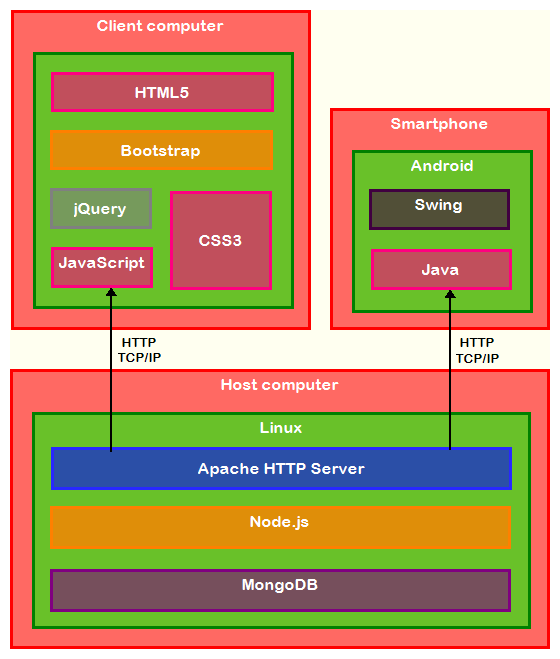
\includegraphics[width=10cm]{Ruan_Diagrams/technical_architecture.png}  \\
	\end{center}
	\caption{Technical Architecture Diagram}
\end{figure}
% End of Ruan Klinkert Technologies

\newpage

\section{Functional requirements and application design}
%\lable{sec:funcreq}
In order to represent all of the use cases associated with the system we have divided the system up into sections that will indicate all of the use cases associated with each and how they include or expand upon other use cases.
	
\subsection{Publication subsystem} 
	\subsubsection{Use cases} 
		\begin{figure}[H]
		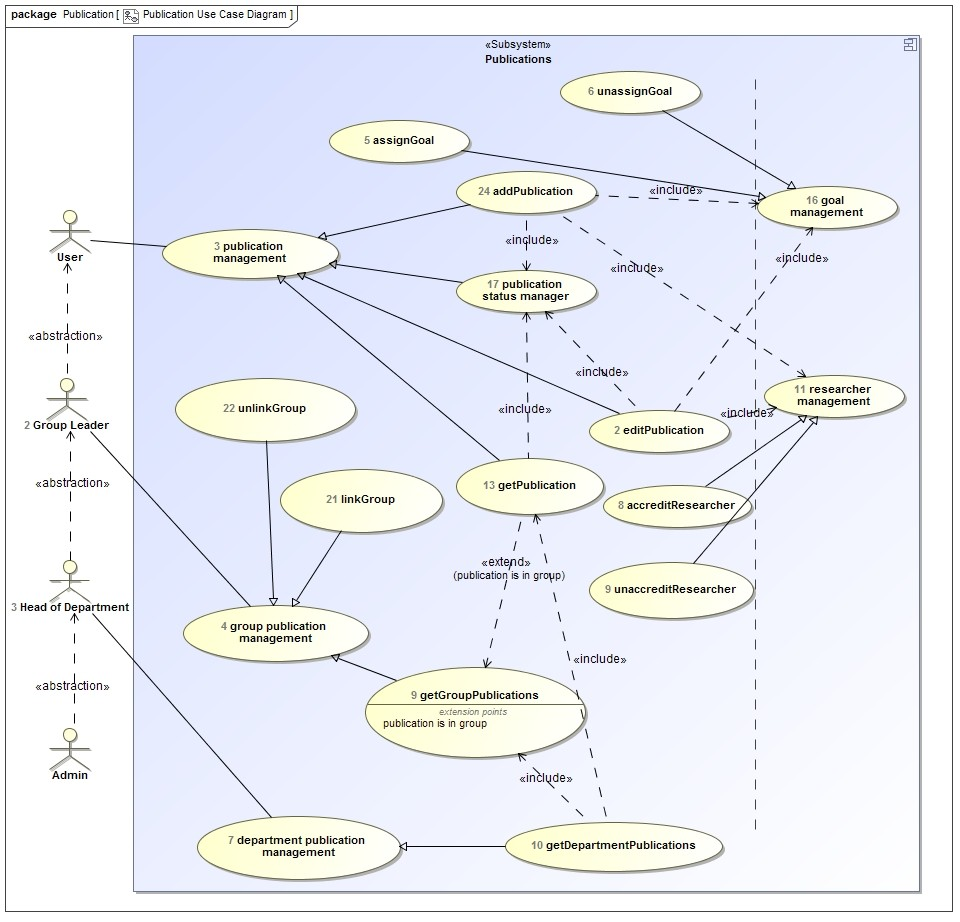
\includegraphics[width=\textwidth]{Quinton_Diagrams/uc__Publication__Publication_Use_Case_Diagram.jpg}  \\
		\caption{Use Case Diagram : Publications}
		\end{figure}

		\begin{figure}[H]
		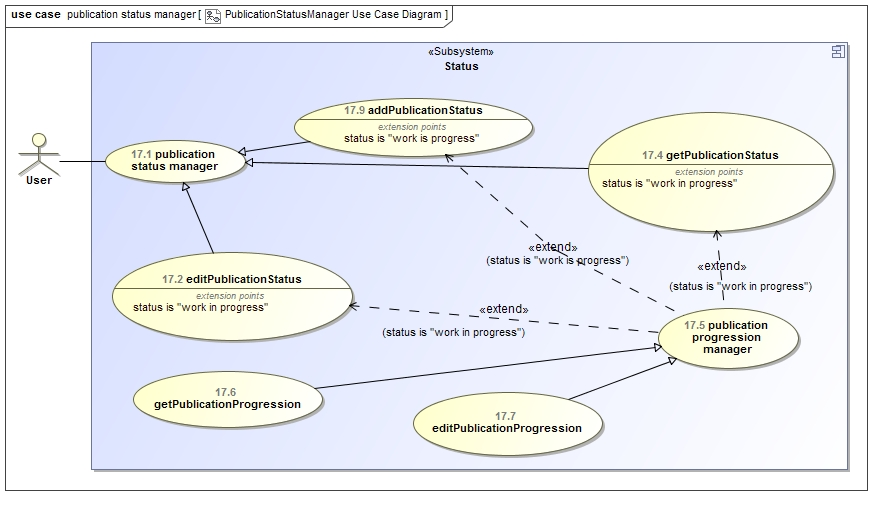
\includegraphics[width=\textwidth]{Quinton_Diagrams/uc__publication_status_manager__PublicationStatusManager_Use_Case_Diagram.jpg}  \\
		\caption{Use Case Diagram : Statuses}
		\end{figure}

		\begin{flushleft}
			\textbf{Critical}
				\begin{itemize}
	  				\item addPublication
	  				\item editPublication
	  				\item getPublication
	  				\item addPublicationStatus
	  				\item getPublicationStatus
	  				\item assignGoal
	  				\item unassignGoal
	  				\item accreditResearcher
	  				\item unaccreditResearcher
	  				\item linkGroup
	  				\item unlinkGroup
				\end{itemize}

			\textbf{Important}
				\begin{itemize}
	  				\item editPublicationStatus
	  				\item getPublicationProgression
	  				\item editPublicationProgression
	  				\item editPublicationStatus
				\end{itemize}

			\textbf{Nice-To-Have}
				\begin{itemize}
	  				\item getDepartmentPublications
	  				\item getGroupPublications
				\end{itemize}
		\end{flushleft}

	\subsubsection{Services Contracts}
		\begin{figure}[H]
		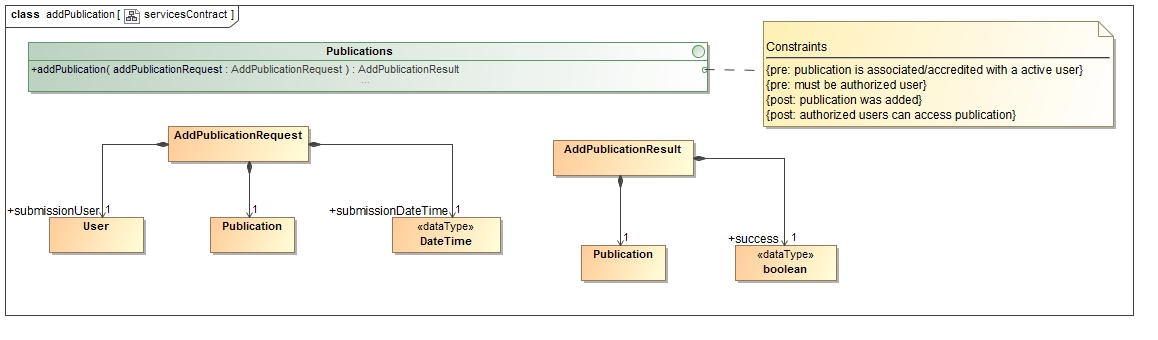
\includegraphics[width=\textwidth]{Quinton_Diagrams/class__addPublication__servicesContract.jpg}  \\
		\caption{Services Contract : addPublication}
		\end{figure}

		\begin{figure}[H]
		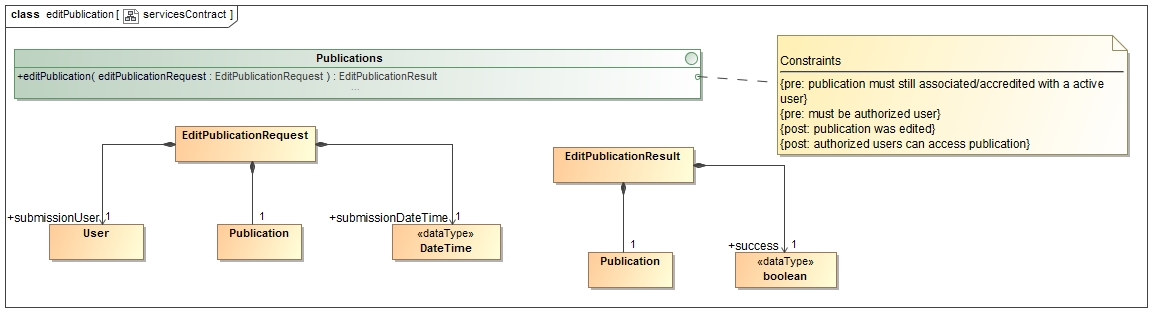
\includegraphics[width=\textwidth]{Quinton_Diagrams/class__editPublication__servicesContract.jpg}  \\
		\caption{Services Contract : editPublication}
		\end{figure}
		
		\begin{figure}[H]
		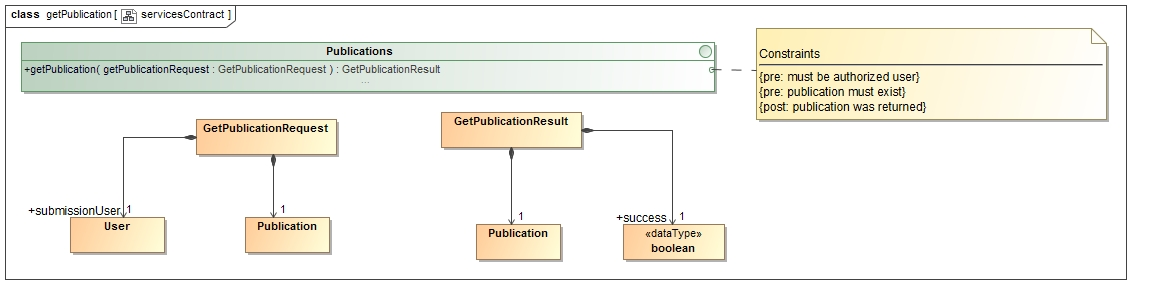
\includegraphics[width=\textwidth]{Quinton_Diagrams/class__getPublication__servicesContract.jpg}  \\
		\caption{Services Contract : getPublication}
		\end{figure}
		
		\begin{figure}[H]
		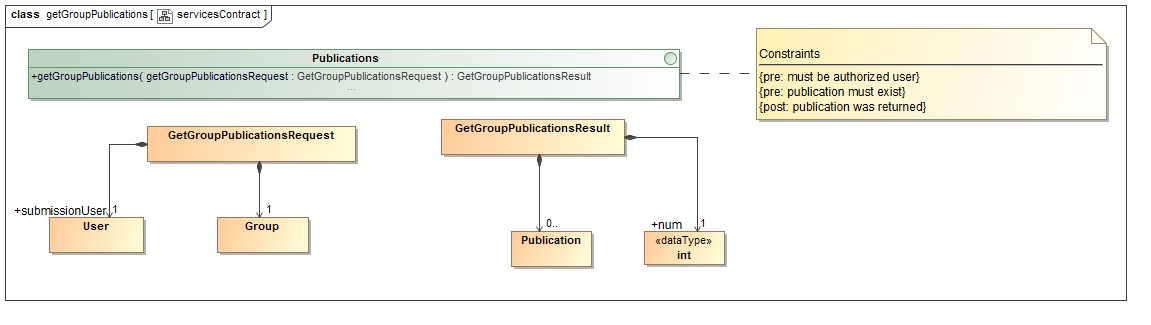
\includegraphics[width=\textwidth]{Quinton_Diagrams/class__getGroupPublications__servicesContract.jpg}  \\
		\caption{Services Contract : getGroupPublications}
		\end{figure}
		
		\begin{figure}[H]
		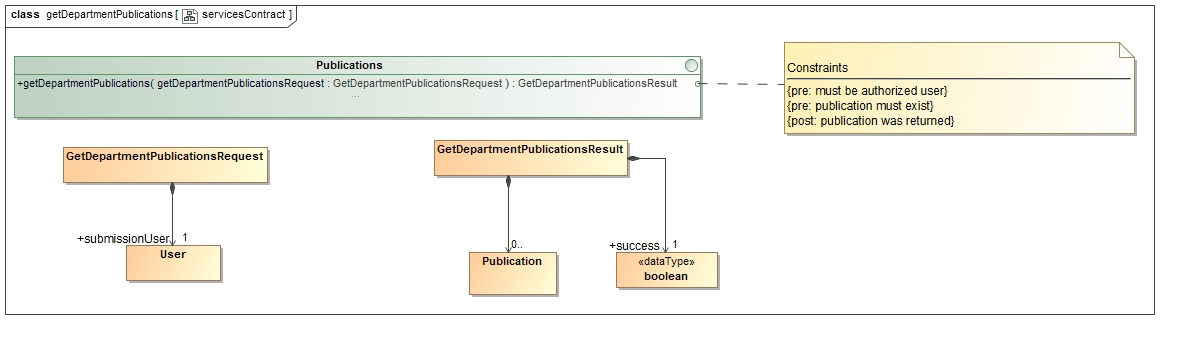
\includegraphics[width=\textwidth]{Quinton_Diagrams/class__getDepartmentPublications__servicesContract.jpg}  \\
		\caption{Services Contract : getDepartmentPublications}
		\end{figure}
		
		\begin{figure}[H]
		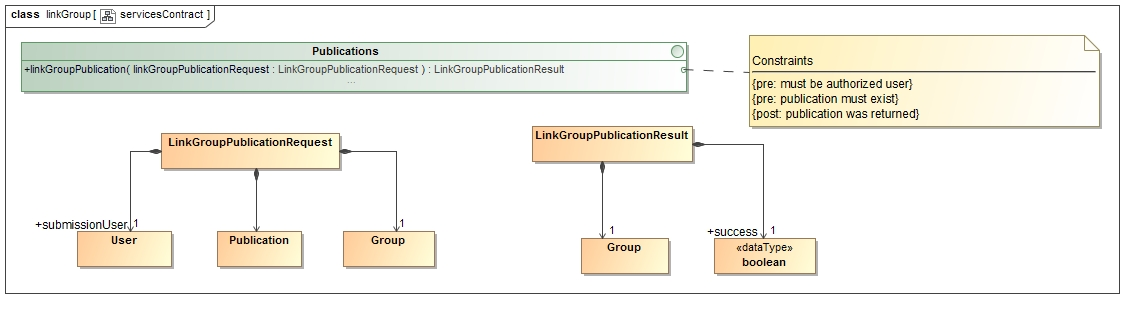
\includegraphics[width=\textwidth]{Quinton_Diagrams/class__linkGroup__servicesContract.jpg}  \\
		\caption{Services Contract : linkGroup}
		\end{figure}
		
		\begin{figure}[H]
		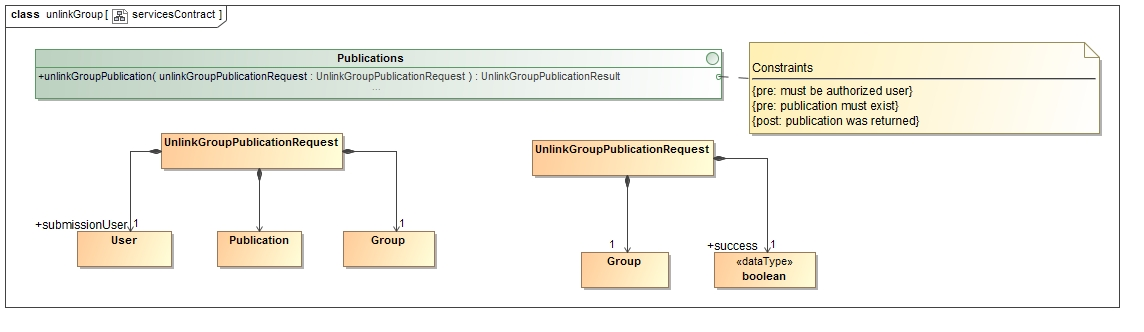
\includegraphics[width=\textwidth]{Quinton_Diagrams/class__unlinkGroup__servicesContract.jpg}  \\
		\caption{Services Contract : unlinkGroup}
		\end{figure}
		
		%Status Manager
		\begin{figure}[H]
		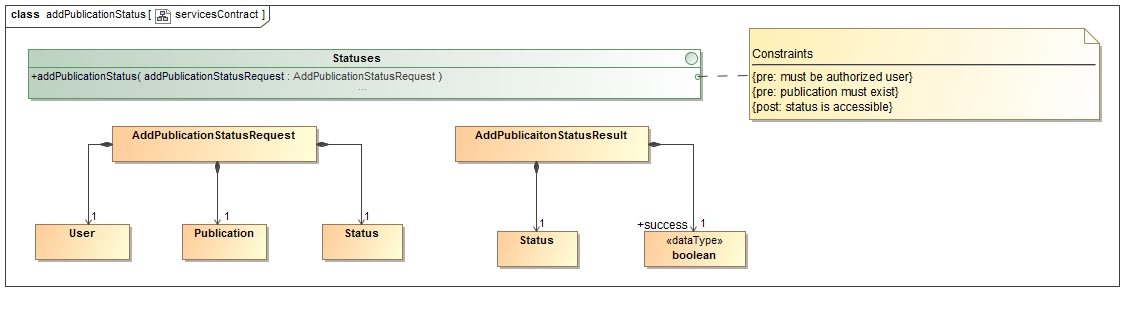
\includegraphics[width=\textwidth]{Quinton_Diagrams/class__addPublicationStatus__servicesContract.jpg}  \\
		\caption{Services Contract : addPublicationStatus}
		\end{figure}
		
		\begin{figure}[H]
		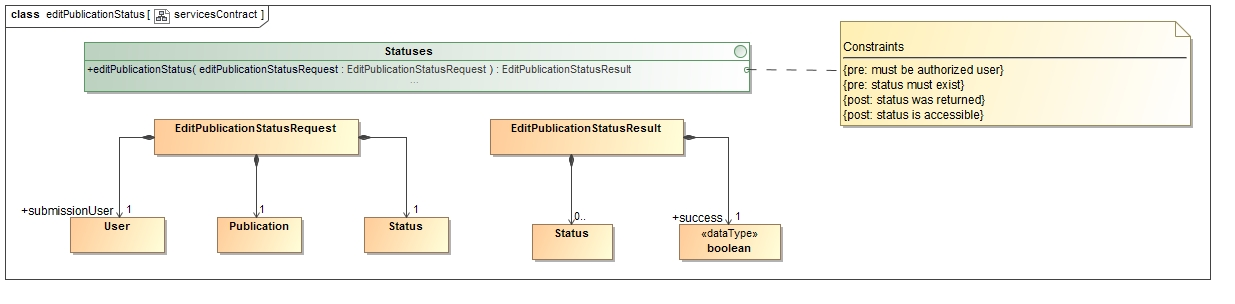
\includegraphics[width=\textwidth]{Quinton_Diagrams/class__editPublicationStatus__servicesContract.jpg}  \\
		\caption{Services Contract : editPublicationStatus}
		\end{figure}
		
		\begin{figure}[H]
		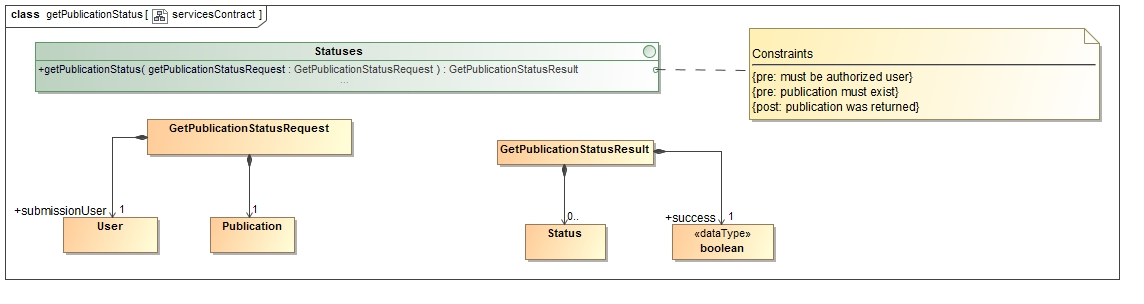
\includegraphics[width=\textwidth]{Quinton_Diagrams/class__getPublicationStatus__servicesContract.jpg}  \\
		\caption{Services Contract : getPublicationStatus}
		\end{figure}
		

	\subsubsection{Required Functionality}
		\begin{figure}[H]
		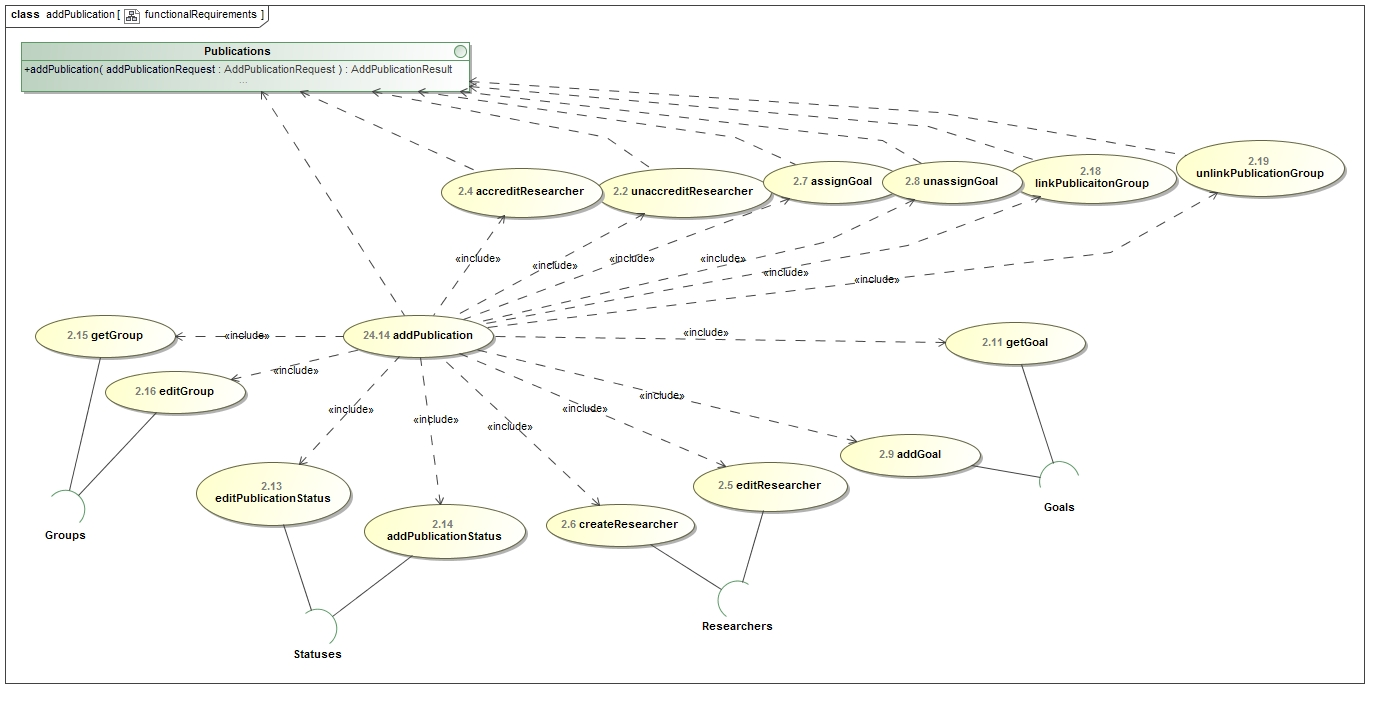
\includegraphics[width=\textwidth]{Quinton_Diagrams/class__addPublication__functionalRequirements.jpg}  \\
		\caption{Functional Requirements : addPublication}
		\end{figure}
		
		\begin{figure}[H]
		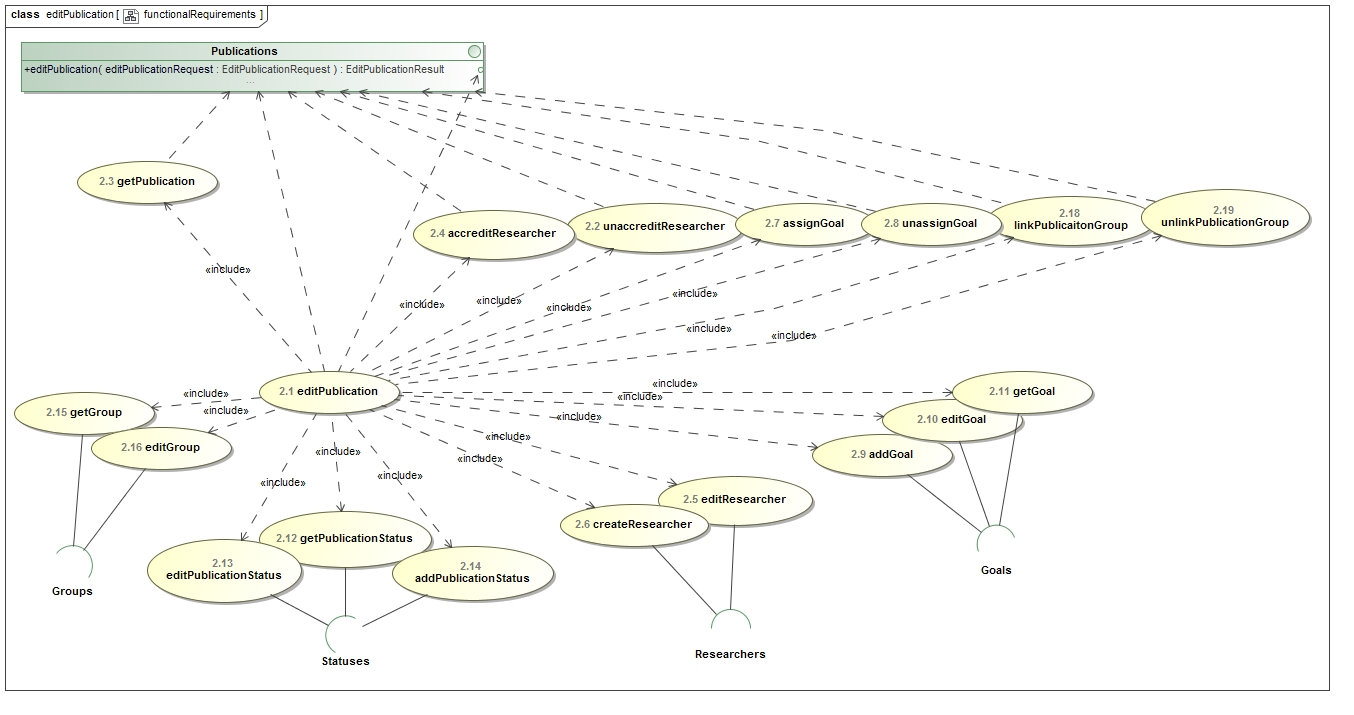
\includegraphics[width=\textwidth]{Quinton_Diagrams/class__editPublication__functionalRequirements.jpg}  \\
		\caption{Functional Requirements : editPublication}
		\end{figure}
		
		\begin{figure}[H]
		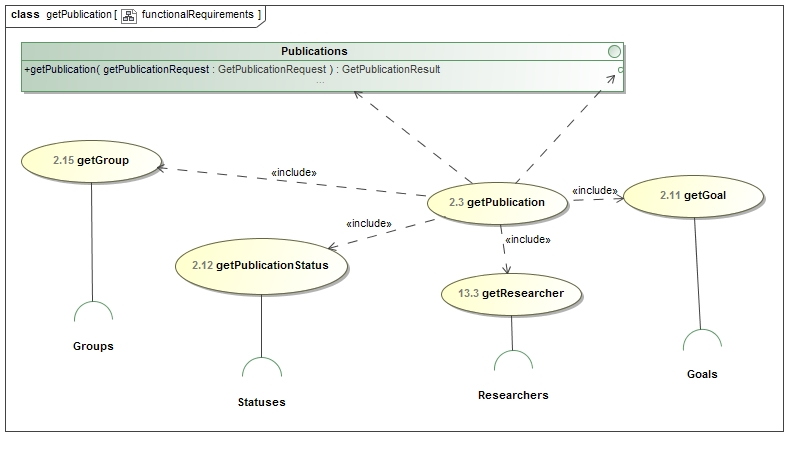
\includegraphics[width=16cm]{Quinton_Diagrams/class__getPublication__functionalRequirements.jpg}  \\
		\caption{Functional Requirements : getPublication}
		\end{figure}
		
		\begin{figure}[H]
		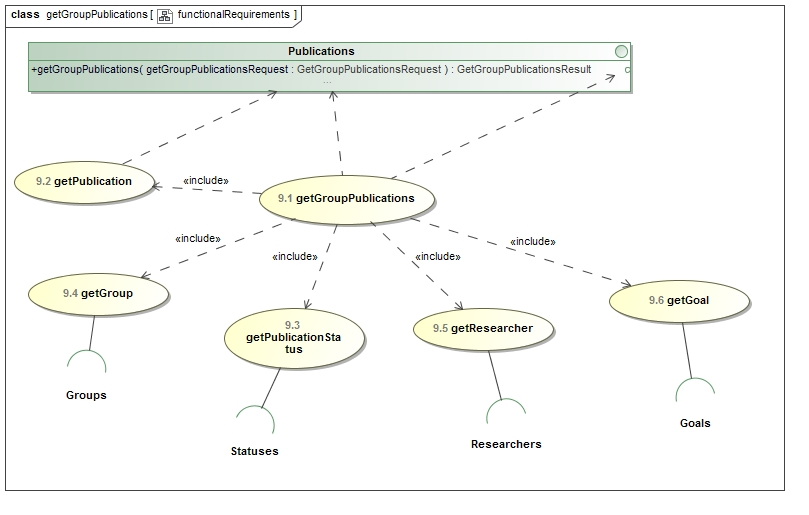
\includegraphics[width=16cm]{Quinton_Diagrams/class__getGroupPublications__functionalRequirements.jpg}  \\
		\caption{Functional Requirements : getGroupPublications}
		\end{figure}
		
		\begin{figure}[H]
		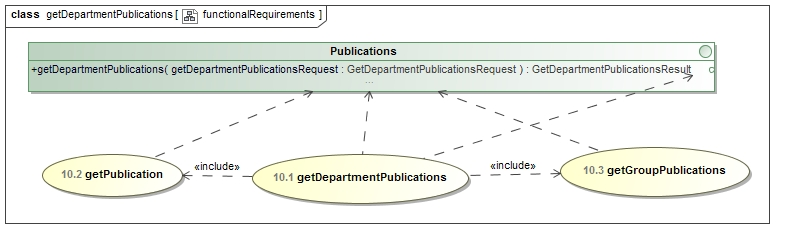
\includegraphics[width=\textwidth]{Quinton_Diagrams/class__getDepartmentPublications__functionalRequirements.jpg}  \\
		\caption{Functional Requirements : getDepartmentPublications}
		\end{figure}
		
		\begin{figure}[H]
		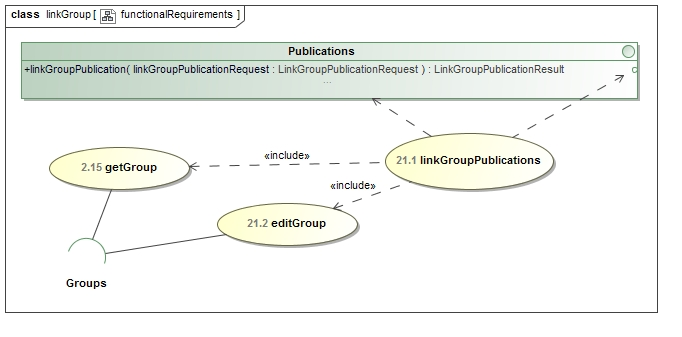
\includegraphics[width=\textwidth]{Quinton_Diagrams/class__linkGroup__functionalRequirements.jpg}  \\
		\caption{Functional Requirements : linkGroup}
		\end{figure}
		
		\begin{figure}[H]
		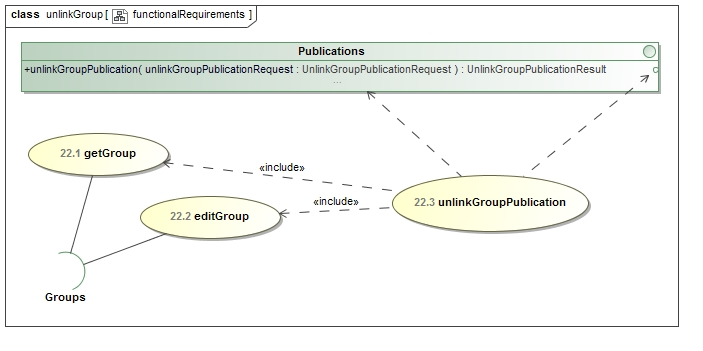
\includegraphics[width=\textwidth]{Quinton_Diagrams/class__unlinkGroup__functionalRequirements.jpg}  \\
		\caption{Functional Requirements : unlinkGroup}
		\end{figure}
		
		%Status Manager
		\begin{figure}[H]
		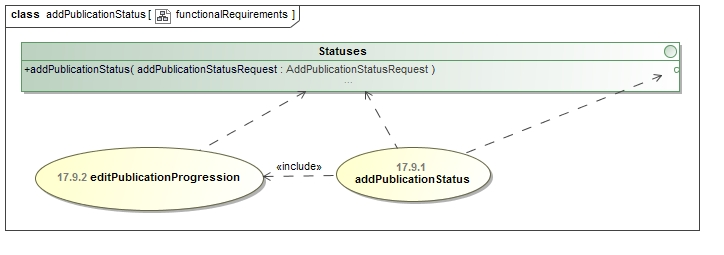
\includegraphics[width=\textwidth]{Quinton_Diagrams/class__addPublicationStatus__functionalRequirements.jpg}  \\
		\caption{Functional Requirements : addPublicationStatus}
		\end{figure}
		
		\begin{figure}[H]
		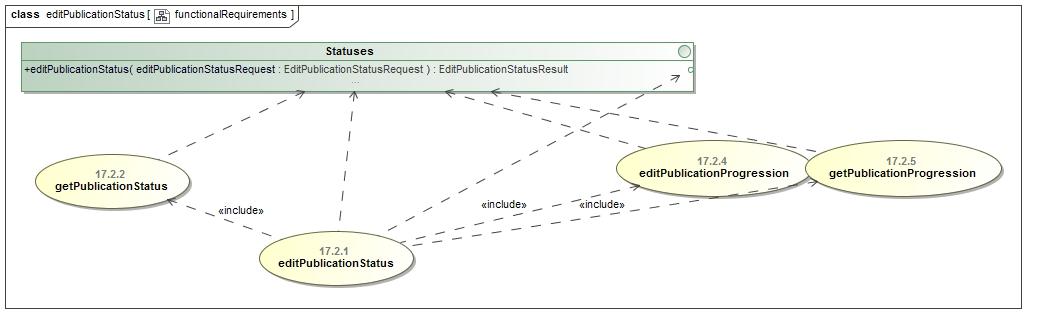
\includegraphics[width=\textwidth]{Quinton_Diagrams/class__editPublicationStatus__functionalRequirements.jpg}  \\
		\caption{Functional Requirements : editPublicationStatus}
		\end{figure}
		
		\begin{figure}[H]
		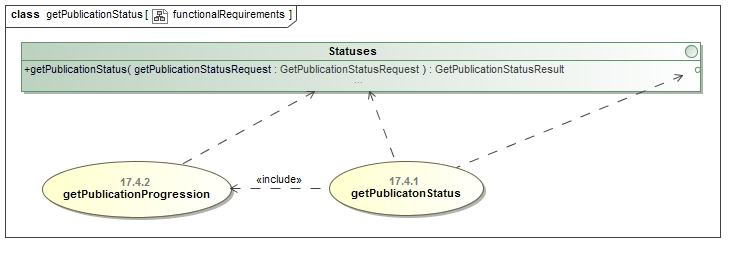
\includegraphics[width=\textwidth]{Quinton_Diagrams/class__getPublicationStatus__functionalRequirements.jpg}  \\
		\caption{Functional Requirements : getPublicationStatus}
		\end{figure}
		

	\subsubsection{Process specifications}
		\begin{figure}[H]
		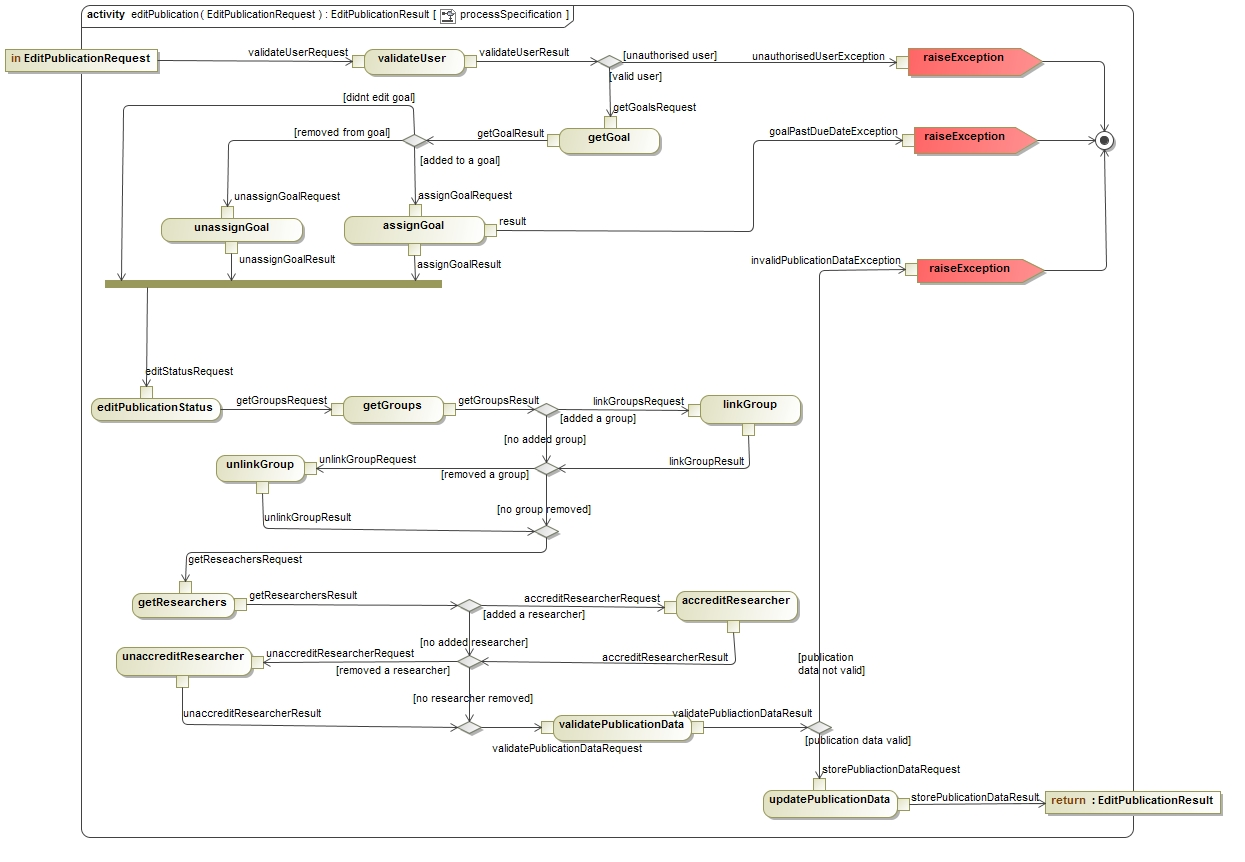
\includegraphics[width=\textwidth]{Quinton_Diagrams/act__editPublication__processSpecification.jpg}  \\
		\caption{Process Specification : editPublicaton}
		\end{figure}
		
		\begin{figure}[H]
		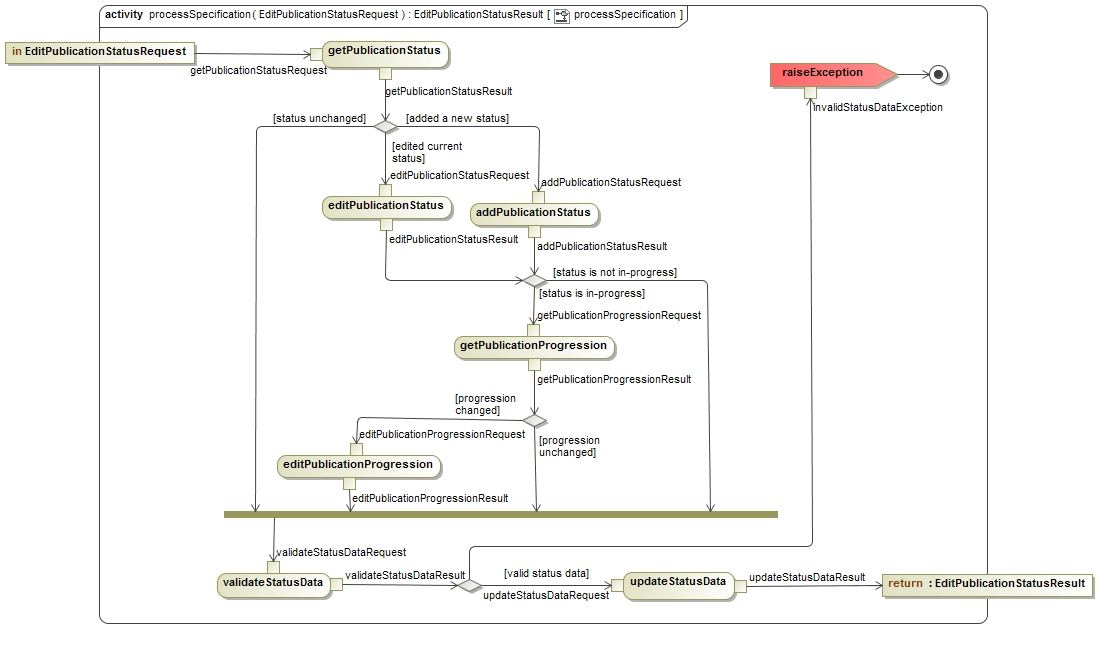
\includegraphics[width=\textwidth]{Quinton_Diagrams/act__processSpecification__processSpecification.jpg}  \\
		\caption{Process Specification : editStatus}
		\end{figure}
		


%Reinhardt Cromhout
\subsection{User subsystem}
	\subsubsection{Use cases}
		\begin{figure}[H]
				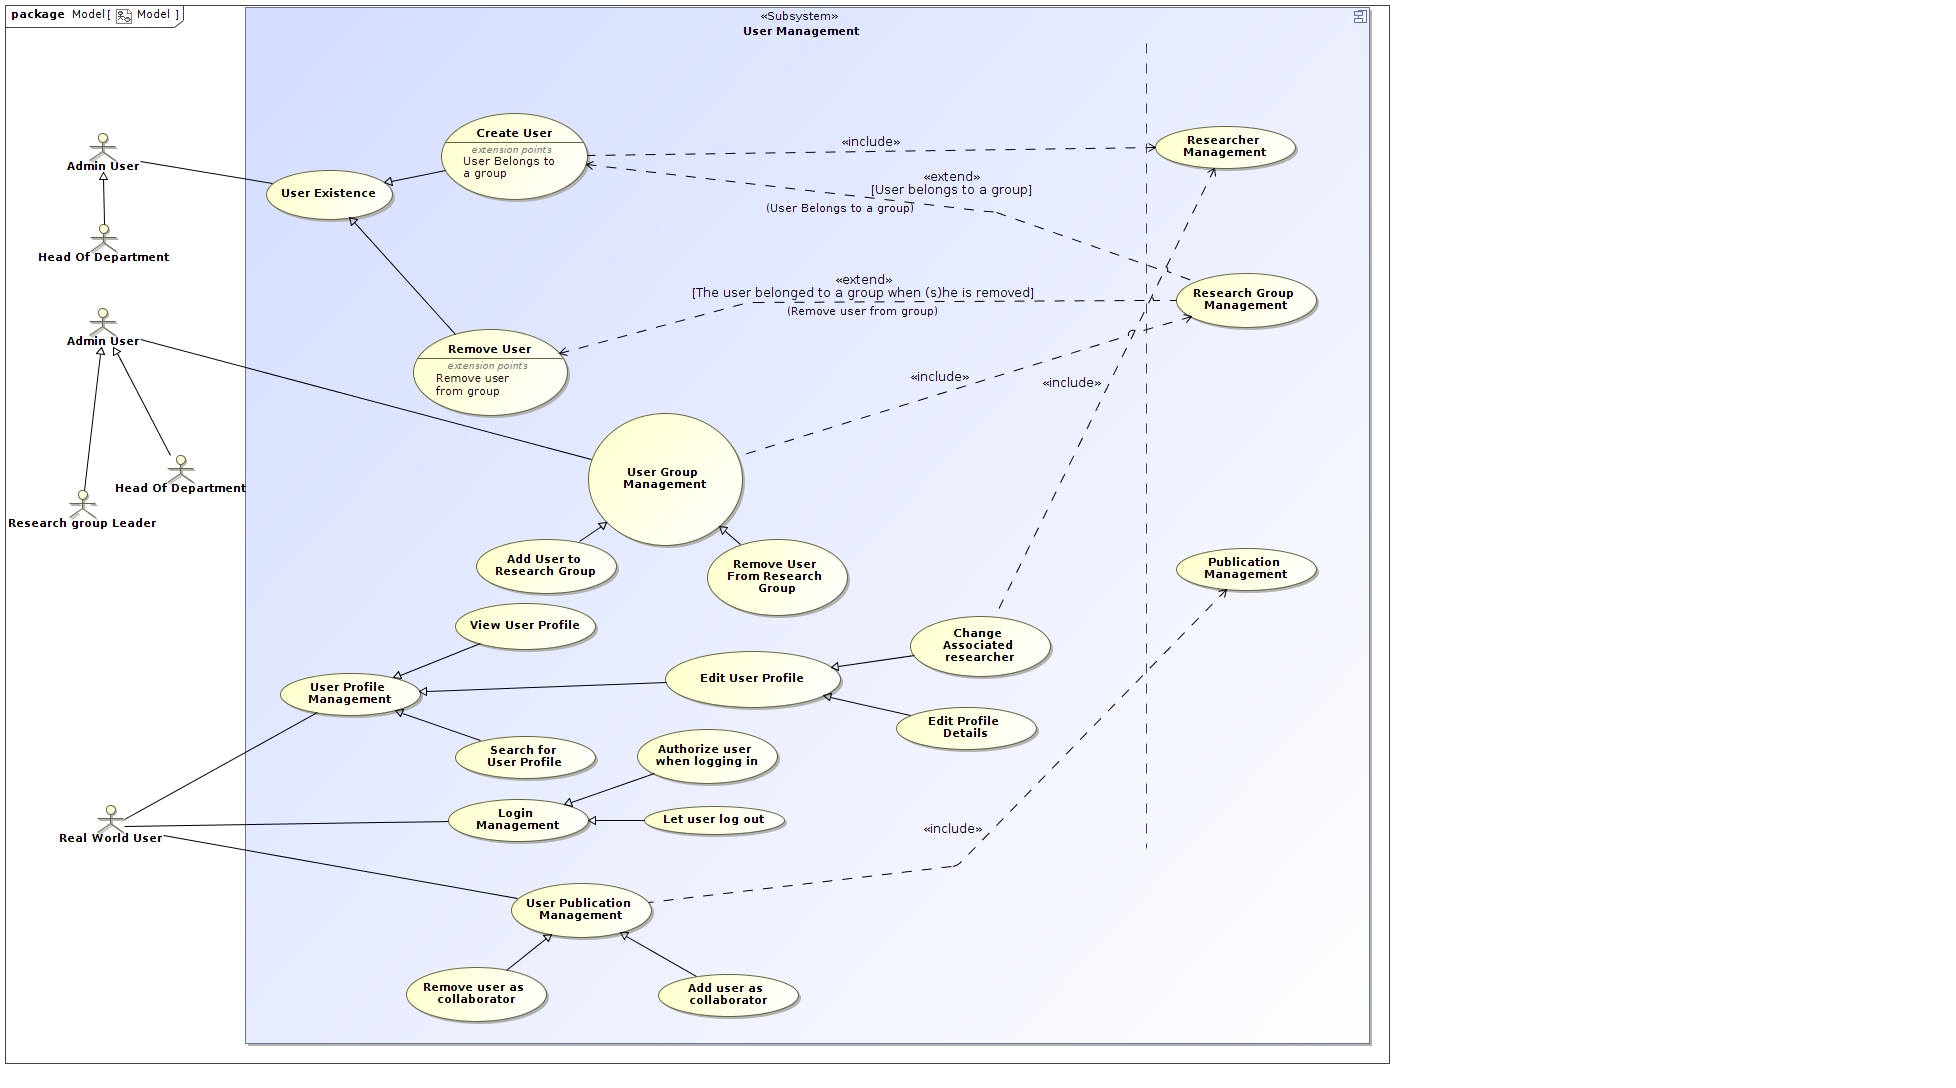
\includegraphics[width=1.5\linewidth]{ReinhardtImages/UserManagement.jpg}
				\caption{The Genereal Use Case Diagram For the User Package}
		  		\label{UseCaseDiagram_UserManagement}
			\end{figure}
			\begin{flushleft}
				\textbf{Critical}
					\begin{itemize}
		  				\item Create User
		 	 			\item User Publication Management
		  				\item Login Management
		  				\item Search for user profile
		  				\item Edit User Profile
					\end{itemize}

				\textbf{Important}
					\begin{itemize}
		  				\item Remove User
		  				\item User Group Management
					\end{itemize}

				\textbf{Nice-To-Have}
					\begin{itemize}
		  				\item View User Profile  				
					\end{itemize}
			\end{flushleft}

	\subsubsection{Services Contracts}
		\begin{figure}[H]
			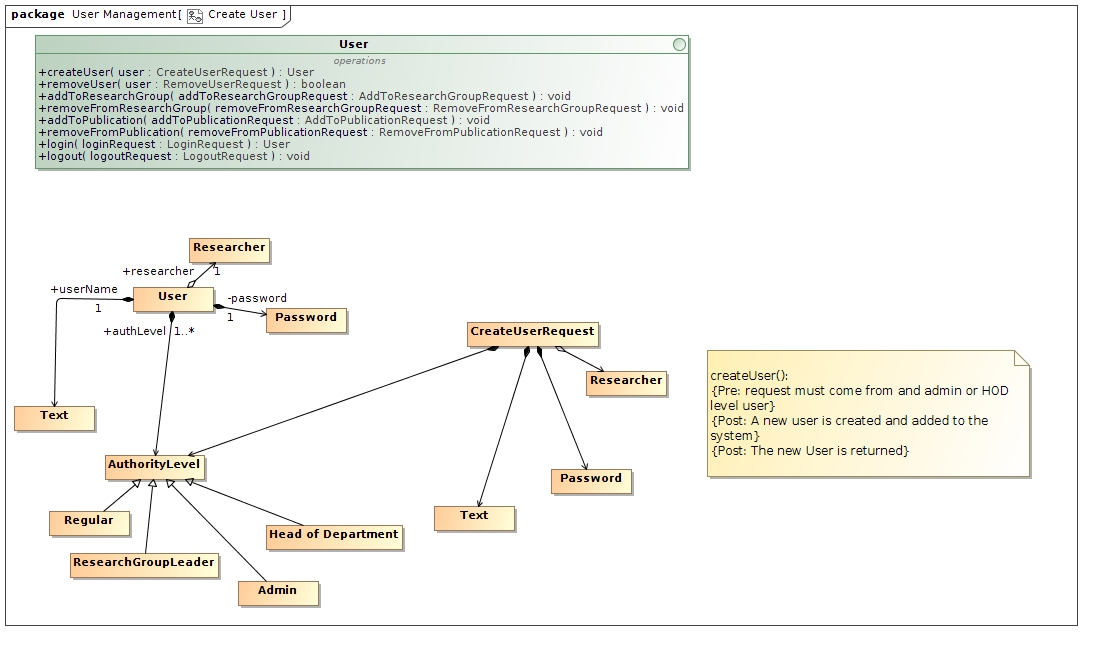
\includegraphics[scale=0.4]{ReinhardtImages/createUser.jpg}
			\caption{Use Case : Create User}
	  		\label{Use Case : Create User}
		\end{figure}
		\begin{figure}[H]
			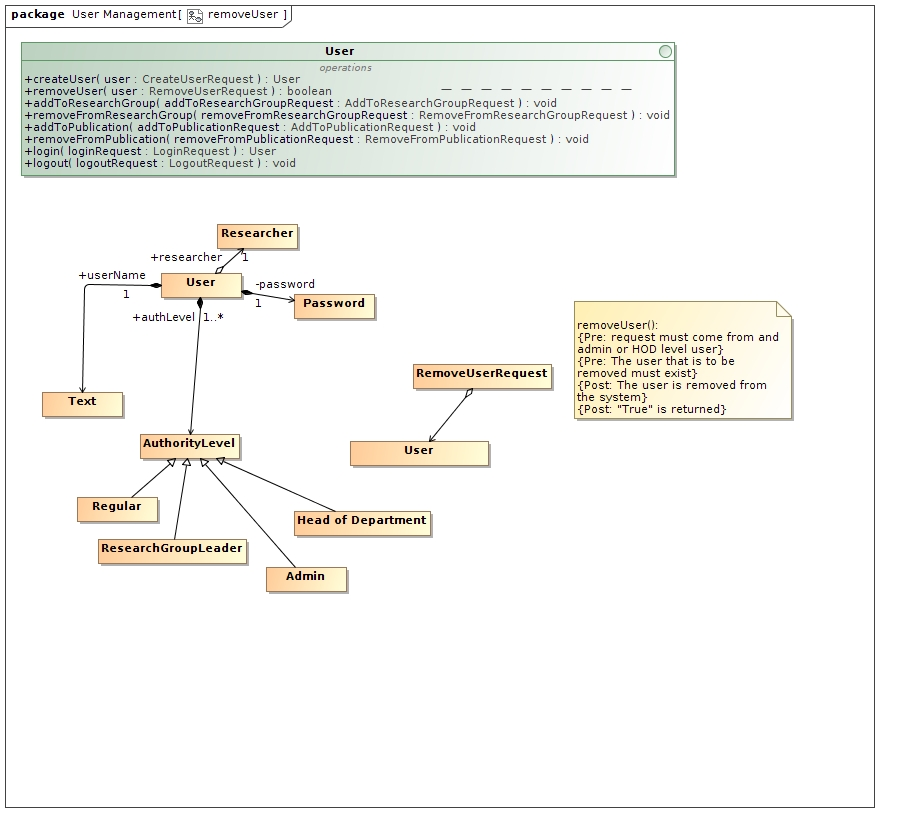
\includegraphics[scale=0.6]{ReinhardtImages/removeUser.jpg}
			\caption{Use Case : Remove User}
	  		\label{Use Case : Remove User}
		\end{figure}
		\begin{figure}[H]
			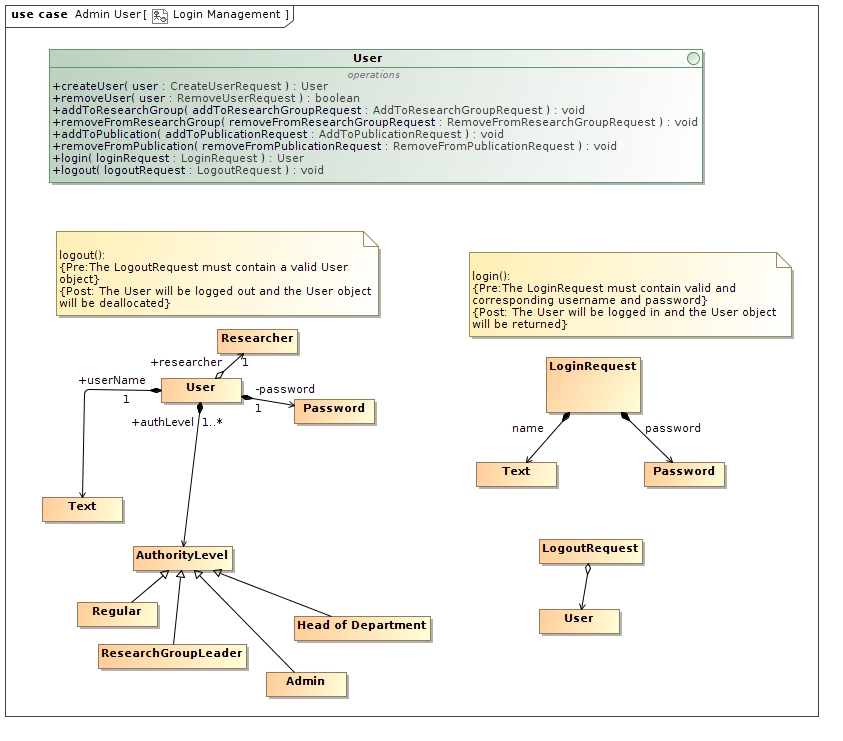
\includegraphics[scale=0.6]{ReinhardtImages/Login Management.jpg}
			\caption{Use Case : Login Management}
	  		\label{Use Case : Login Management}
		\end{figure}
		\begin{figure}[H]
			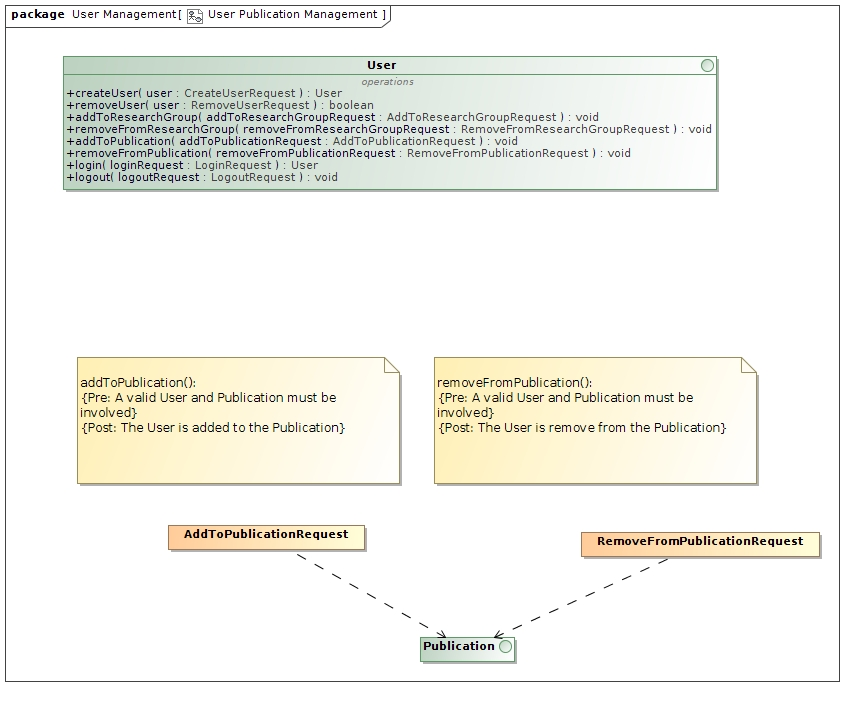
\includegraphics[scale=0.6]{ReinhardtImages/User Publication Management.jpg}
			\caption{Use Case : Publication Management}
	  		\label{Use Case : Publication Management}
		\end{figure}
		\begin{figure}[H]
			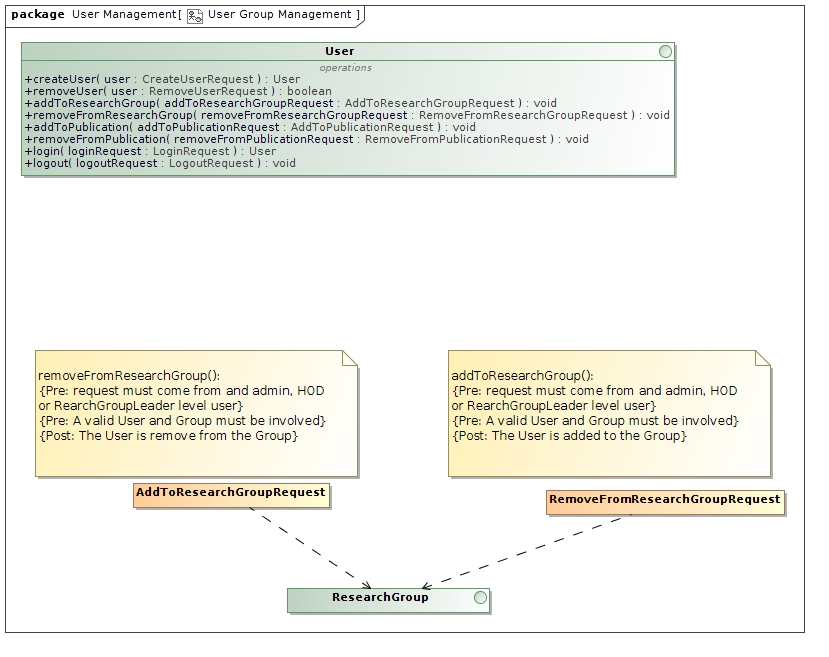
\includegraphics[scale=0.6]{ReinhardtImages/User Group Management.jpg}
			\caption{Use Case : Research Group Management}
	  		\label{Use Case : Research Group Management}
		\end{figure}
		\begin{figure}[H]
			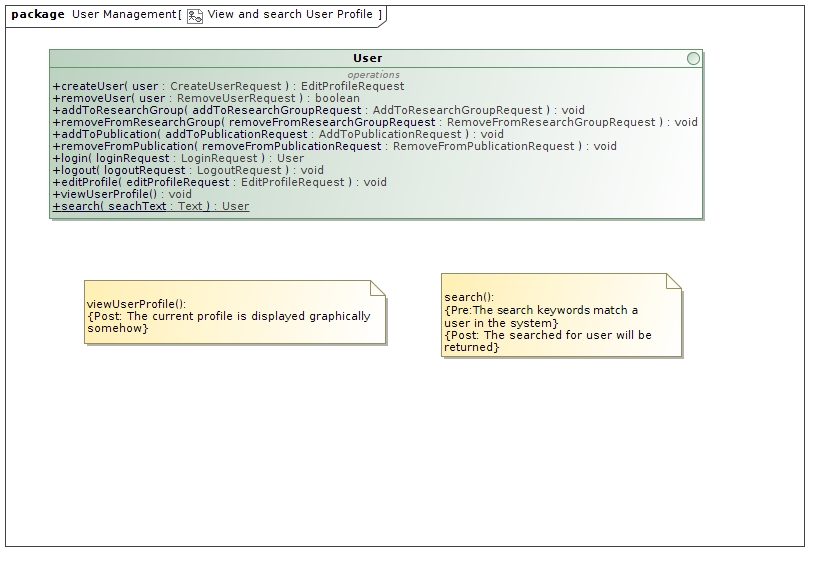
\includegraphics[scale=0.6]{ReinhardtImages/View and search User Profile.jpg}
			\caption{Use Case : View and Search User Profile}
	  		\label{Use Case : View and Search User Profile}
		\end{figure}
		\begin{figure}[H]
			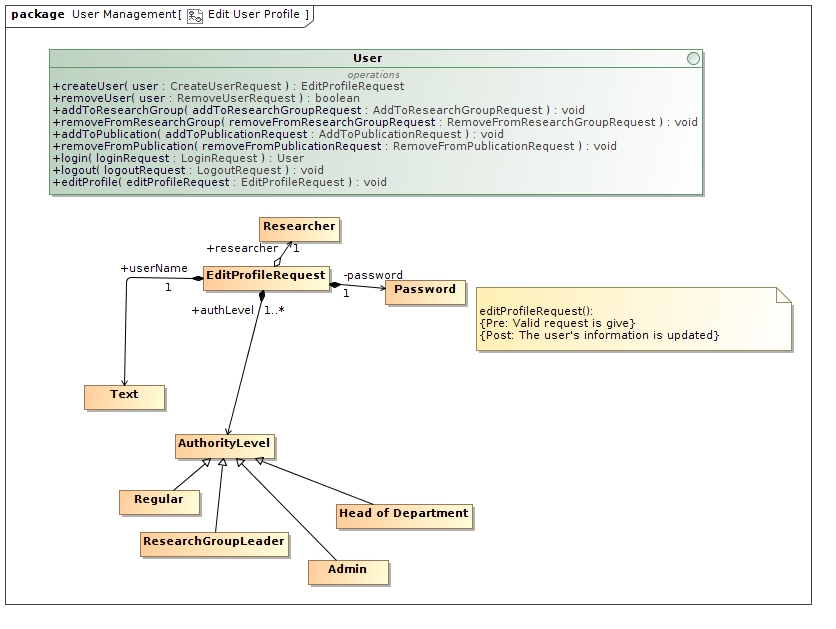
\includegraphics[scale=0.6]{ReinhardtImages/Edit User Profile.jpg}
			\caption{Use Case : Edit User Profile}
	  		\label{Use Case : Edit User Profile}
		\end{figure}		  	

	\subsubsection{Required Functionality}
		\begin{figure}[H]
			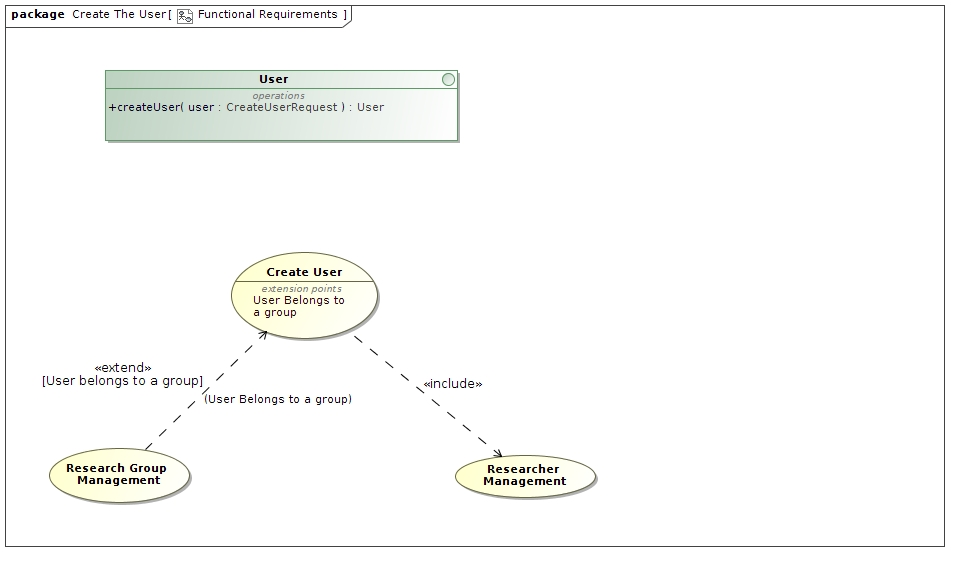
\includegraphics[scale=0.5]{ReinhardtImages/Functional RequirementsCreateUser.jpg}
			\caption{Functional Requirements : Create User}
	  		\label{Functional Requirements : Create User}
		\end{figure}
		\begin{figure}[H]
			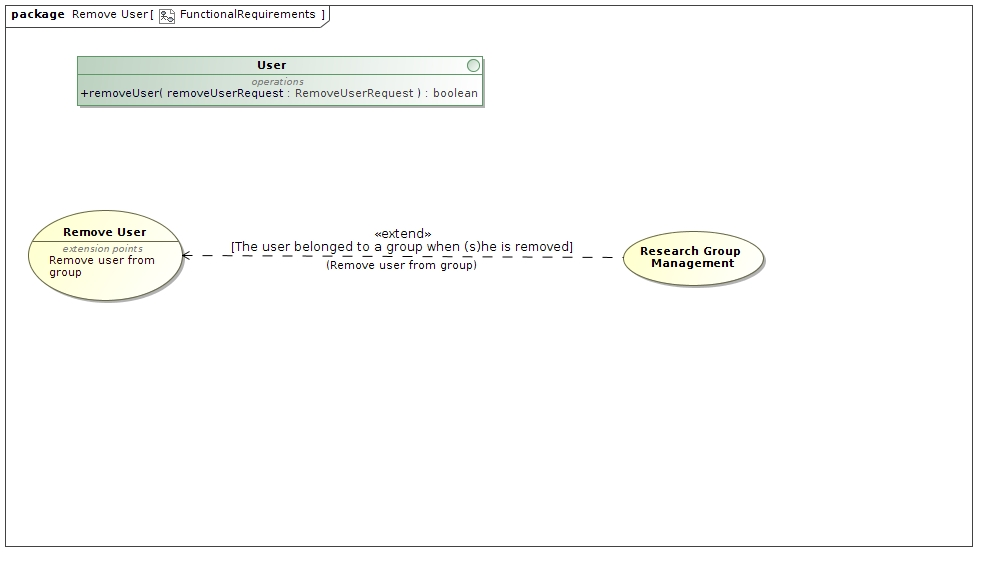
\includegraphics[scale=0.5]{ReinhardtImages/FunctionalRequirementsRemoveUser.jpg}
			\caption{Functional Requirements : Remove User}
	  		\label{Functional Requirements : Remove User}
		\end{figure}
		\begin{figure}[H]
			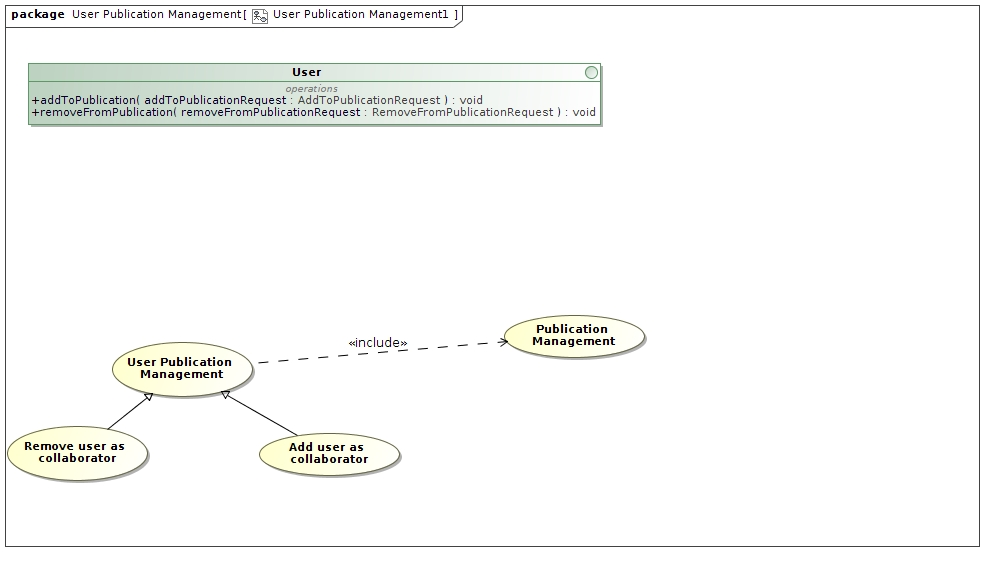
\includegraphics[scale=0.5]{ReinhardtImages/FunctionalRequirementsPublicationManagement.jpg}
			\caption{Functional Requirements : Publication Management}
	  		\label{Functional Requirements : Publication Management}
		\end{figure}
		\begin{figure}[H]
			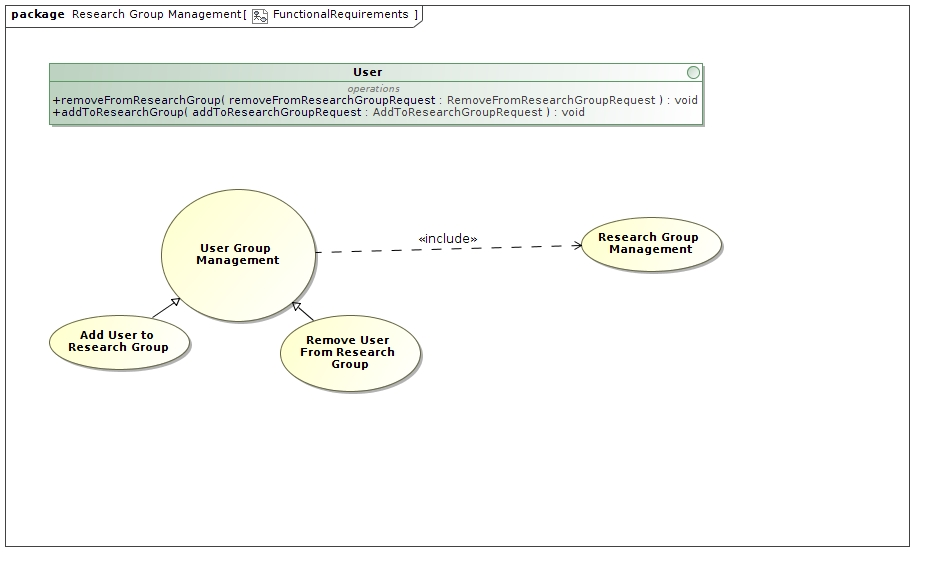
\includegraphics[scale=0.5]{ReinhardtImages/FunctionalRequirementsResearchGroupManagement.jpg}
			\caption{Functional Requirements : Research Group Management}
	  		\label{Functional Requirements : Research Group Management}
		\end{figure}
		\begin{figure}[H]
			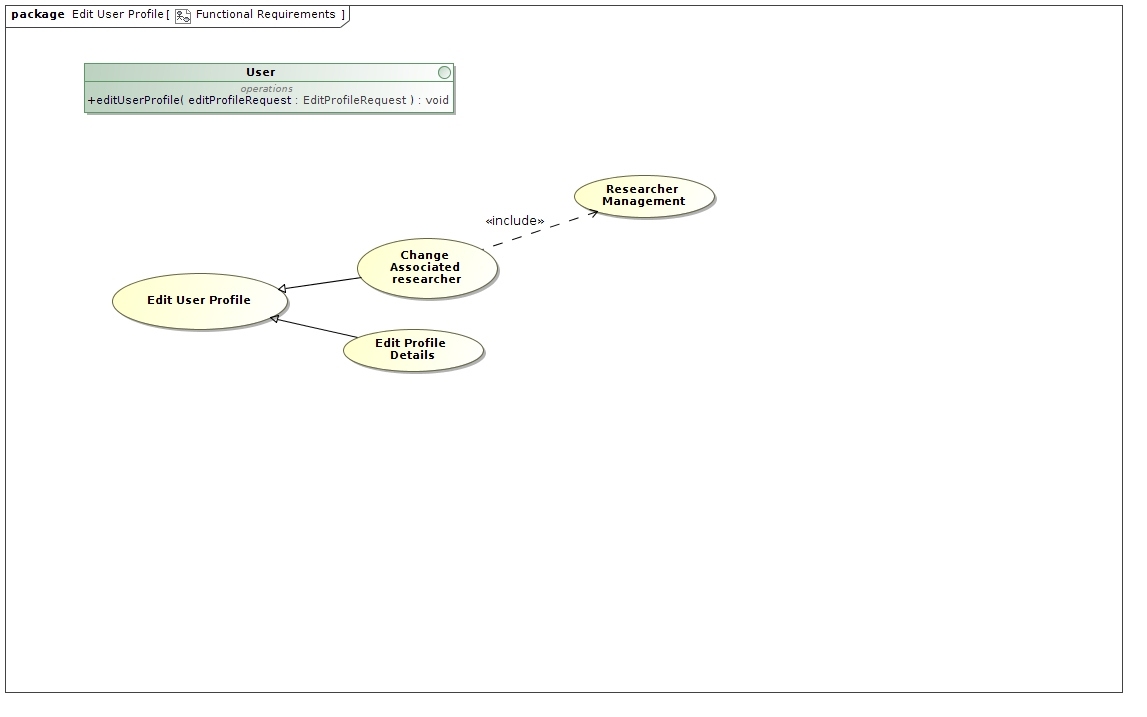
\includegraphics[scale=0.45]{ReinhardtImages/Functional RequirementsEditUserProfile.jpg}
			\caption{Functional Requirements : Edit User Profile}
	  		\label{Functional Requirements : Edit User Profile}
		\end{figure}
	
	%Ruan Klinkert
\subsection{Goal subsystem}
	\subsubsection{Use cases}

		\begin{figure}[H]
			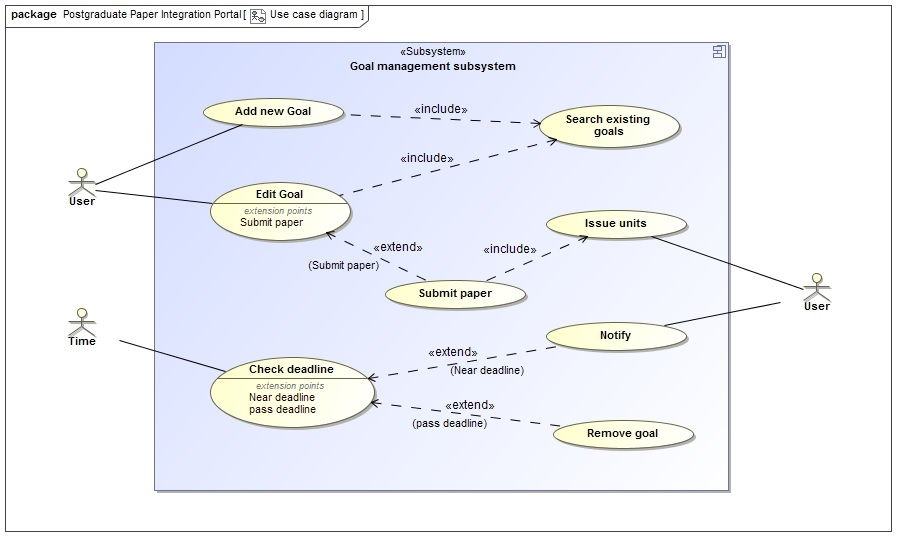
\includegraphics[width=\textwidth]{Ruan_Diagrams/useCaseDiagram.jpg}  \\
			\caption{Use Case Diagram : Postgraduate Paper Integration Portal}
		\end{figure}
		\begin{flushleft}
			\textbf{Critical}
				\begin{itemize}
	  				\item Add new Goal
	 	 			\item Submit paper
	  				\item Edit Goal
				\end{itemize}

			\textbf{Important}
				\begin{itemize}
	  				\item Issue units
	  				\item Remove Goal
				\end{itemize}

			\textbf{Nice-To-Have}
				\begin{itemize}
	  				\item Search existing Goals
	  				\item Notify
	  				\item Check deadline
				\end{itemize}
		\end{flushleft}

	\subsubsection{Services Contracts}

		\begin{figure}[H]
			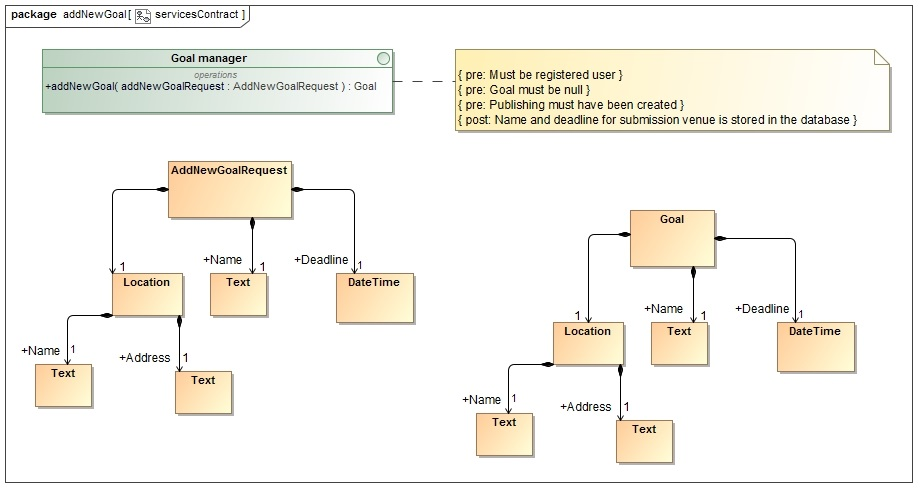
\includegraphics[width=\textwidth]{Ruan_Diagrams/addNewGoal_servicesContract.jpg}  \\
			\caption{Services Contract : addNewGoal}
		\end{figure}
		\begin{figure}[H]
			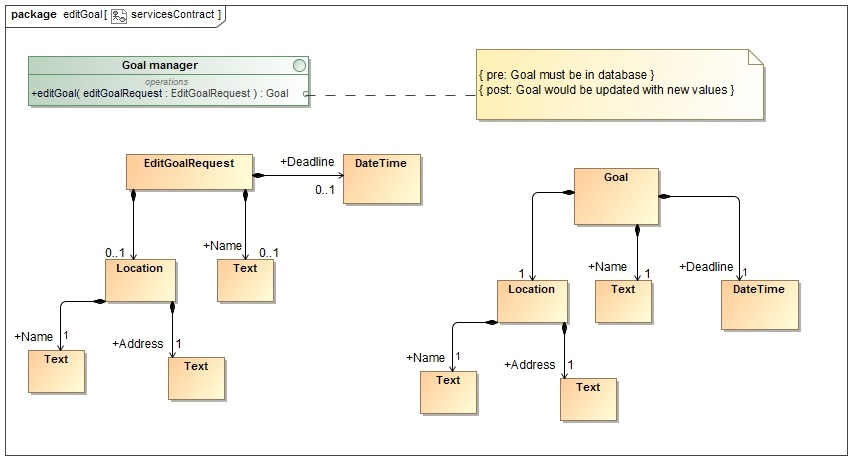
\includegraphics[width=\textwidth]{Ruan_Diagrams/editGoal_servicesContract.jpg}  \\
			\caption{Services Contract : editGoal}
		\end{figure}
		\begin{figure}[H]
			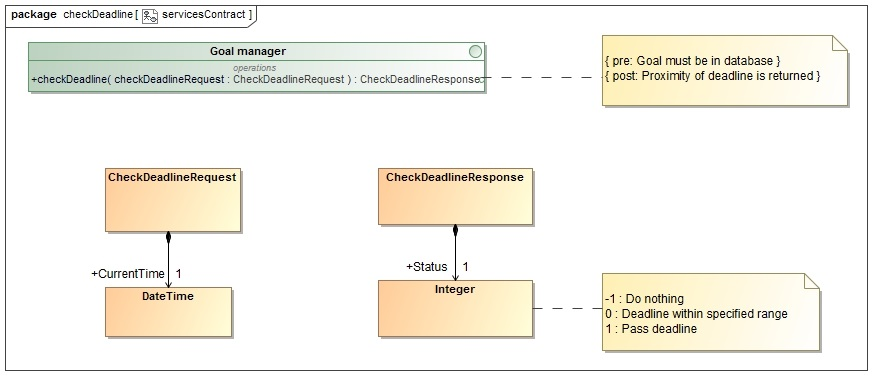
\includegraphics[width=\textwidth]{Ruan_Diagrams/checkDeadline_servicesContract.jpg}  \\
			\caption{Services Contract : checkDeadline}
		\end{figure}
		\begin{figure}[H]
			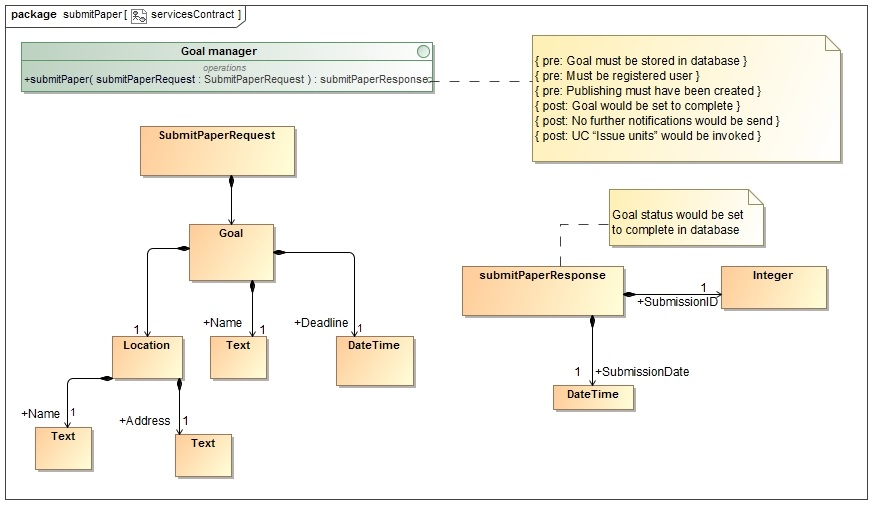
\includegraphics[width=\textwidth]{Ruan_Diagrams/submitPaper_servicesContract.jpg}  \\
			\caption{Services Contract : submitPaper}
		\end{figure}
		\begin{figure}[H]
			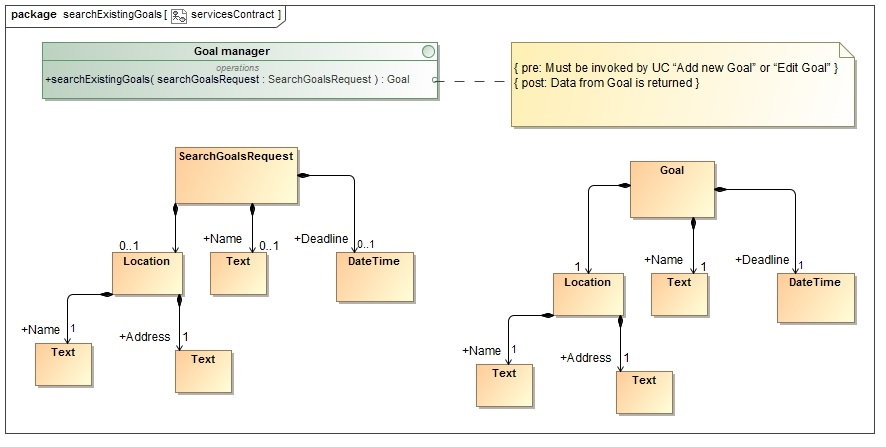
\includegraphics[width=\textwidth]{Ruan_Diagrams/searchExistingGoals_servicesContract.jpg}  \\
			\caption{Services Contract : searchExistingGoals}
		\end{figure}
		\begin{figure}[H]
			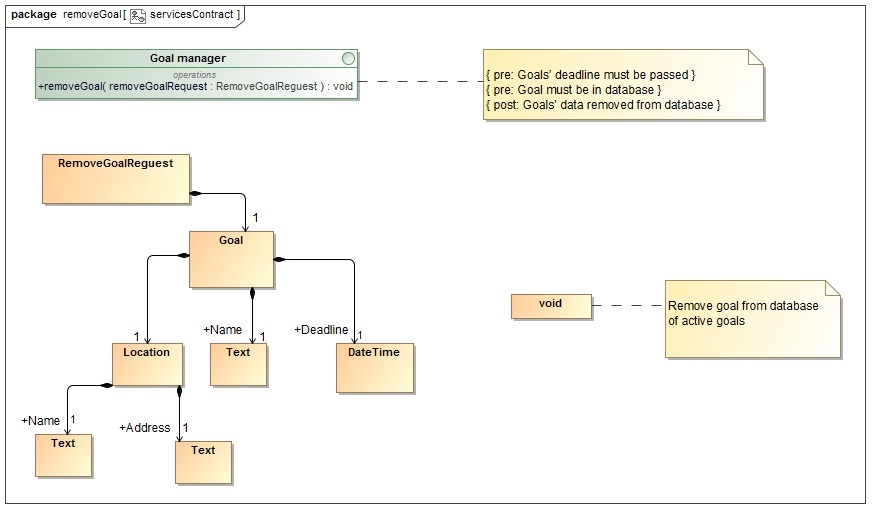
\includegraphics[width=\textwidth]{Ruan_Diagrams/removeGoal_servicesContract.jpg}  \\
			\caption{Services Contract : removeGoal}
		\end{figure}
		\begin{figure}[H]
			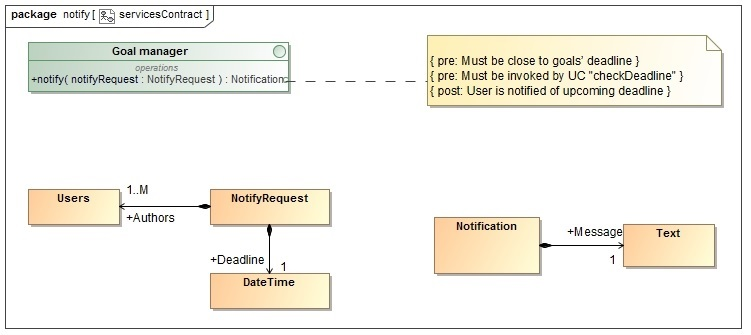
\includegraphics[width=\textwidth]{Ruan_Diagrams/notify_servicesContract.jpg}  \\
			\caption{Services Contract : notify}
		\end{figure}
		\begin{figure}[H]
			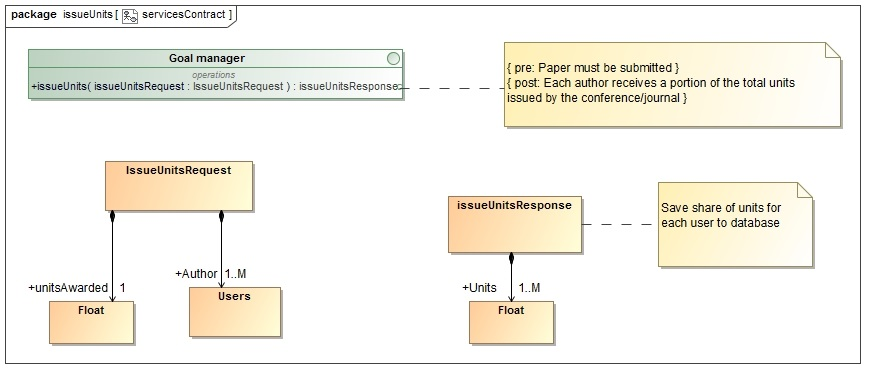
\includegraphics[width=\textwidth]{Ruan_Diagrams/issueUnits_servicesContract.jpg}  \\
			\caption{Services Contract : issueUnits}
		\end{figure}

	\subsubsection{Required functionality}
	
		\begin{figure}[H]
			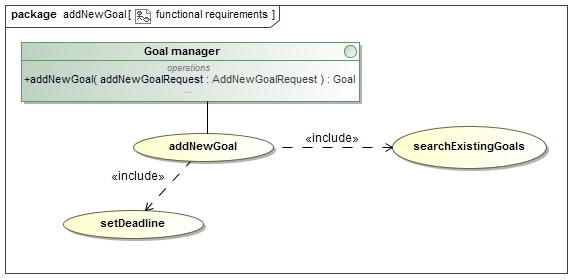
\includegraphics[width=\textwidth]{Ruan_Diagrams/addNewGoal_functionalRequirements.jpg}  \\
			\caption{Functional Requirements : addNewGoal}
		\end{figure}
		\begin{figure}[H]
			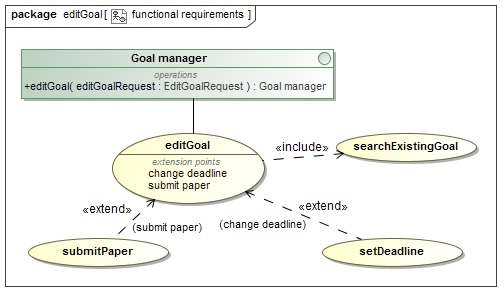
\includegraphics[width=\textwidth]{Ruan_Diagrams/editGoal_functionalRequirements.jpg}  \\
			\caption{Functional Requirements : editGoal}
		\end{figure}
		\begin{figure}[H]
			\includegraphics[width=\textwidth]{Ruan_Diagrams/checkDeadline_functionalRequirements.jpg}  \\
			\caption{Functional Requirements : checkDeadlines}
		\end{figure}
		\begin{figure}[H]
			\includegraphics[width=\textwidth]{Ruan_Diagrams/submitPaper_functionalRequirements.jpg}  \\
			\caption{Functional Requirements : submitPaper}
		\end{figure}
		\begin{figure}[H]
			\includegraphics[width=\textwidth]{Ruan_Diagrams/searchExistingGoals_functionalRequirements.jpg}  \\
			\caption{Functional Requirements : searchExistingGoals}
		\end{figure}
		\begin{figure}[H]
			\includegraphics[width=\textwidth]{Ruan_Diagrams/removeGoal_functionalRequirements.jpg}  \\
			\caption{Functional Requirements : removeGoal}
		\end{figure}
		\begin{figure}[H]
			\includegraphics[width=\textwidth]{Ruan_Diagrams/notify_functionalRequirements.jpg}  \\
			\caption{Functional Requirements : notify}
		\end{figure}
		\begin{figure}[H]
			\includegraphics[width=\textwidth]{Ruan_Diagrams/issueUnits_functionalRequirements.jpg}  \\
			\caption{Functional Requirements : issueUnits}
		\end{figure}
	
	\subsubsection{Process specifications}
	
		\begin{figure}[H]
			\includegraphics[width=\textwidth]{Ruan_Diagrams/addNewGoal_processSpecification.jpg}  \\
			\caption{Process Specification : addNewGoal}
		\end{figure}
		\begin{figure}[H]
			\includegraphics[width=\textwidth]{Ruan_Diagrams/editGoal_processSpecification.jpg}  \\
			\caption{Process Specification : editGoal}
		\end{figure}
		\begin{figure}[H]
			\includegraphics[width=\textwidth]{Ruan_Diagrams/checkdeadline_processSpecification.jpg}  \\
			\caption{Process Specification : checkDeadline}
		\end{figure}
  		\begin{figure}[H]
  			\includegraphics[width=\textwidth]{Ruan_Diagrams/submitPaper_processSpecification.jpg}  \\
  			\caption{Process Specification : submitPaper}
  		\end{figure}
  		\begin{figure}[H]
  			\includegraphics[width=\textwidth]{Ruan_Diagrams/removeGoal_processSpecification.jpg}  \\
  			\caption{Process Specification : removeGoal}
  		\end{figure}
  		\begin{figure}[H]
  			\includegraphics[width=\textwidth]{Ruan_Diagrams/notify_processSpecification.jpg}  \\
  			\caption{Process Specification : notify}
  		\end{figure}
	
	% End of Ruan Klinkert

\subsection{Researcher subsystem}
	\subsubsection{Use cases}
	
		%\includegraphics [width=\textwidth]{uc__Postgraduate_Publication_Interaction_Portal__Publication_Use_Case_Diagram.jpg}  \\
		
		\begin{figure}[H]
			\includegraphics[width=\textwidth]{Rohan_Diagrams/UseCase.jpg}  \\
			\caption{Use Case Diagram : ResearcherManagement}
		\end{figure}

		\begin{flushleft}
			\textbf{Critical}
				\begin{itemize}
	  				\item Add new Researcher
	  				\item Delete Researcher
	  				\item Edit Researcher
				\end{itemize}

			\textbf{Important}
				\begin{itemize}
	  				\item Searching for researcher
	  				\item Checking user authorization
				\end{itemize}

			\textbf{Nice-To-Have}
				\begin{itemize}
	  				\item View Researcher information
				\end{itemize}
		\end{flushleft}

	\subsubsection{Services Contracts}

		%\includegraphics[width=\textwidth]{class.jpg}  \\
		\begin{figure}[H]
			\includegraphics[width=\textwidth]{Rohan_Diagrams/createResearcherServiceContract.jpg}  \\
			\caption{Services Contract : createResearcher}
		\end{figure}
		\begin{figure}[H]
			\includegraphics[width=\textwidth]{Rohan_Diagrams/deleteReseacherServiceContract.jpg}  \\
			\caption{Services Contract : deleteResearcher}
		\end{figure}
		\begin{figure}[H]
			\includegraphics[width=\textwidth]{Rohan_Diagrams/editResearcherServiceContract.jpg}  \\
			\caption{Services Contract : editResearcher}
		\end{figure}
		\begin{figure}[H]
			\includegraphics[width=\textwidth]{Rohan_Diagrams/searchServiceContract.jpg}  \\
			\caption{Services Contract : search}
		\end{figure}

	\subsubsection{Required Functionality}
		
		\begin{figure}[H]
			\includegraphics[width=\textwidth]{Rohan_Diagrams/createResearcherFunctionalRequirements.jpg}  \\
			\caption{Functional Requirements : createResearcher}
		\end{figure}
		\begin{figure}[H]
			\includegraphics[width=\textwidth]{Rohan_Diagrams/deleteResearcherFunctionalRequirements.jpg}  \\
			\caption{Functional Requirements : deleteResearcher}
		\end{figure}
		\begin{figure}[H]
			\includegraphics[width=\textwidth]{Rohan_Diagrams/editResearcherFunctionalRequirements.jpg}  \\
			\caption{Functional Requirements : editResearcher}
		\end{figure}
	
	\subsubsection{Process specifications}
	
		\begin{figure}[H]
			\includegraphics[width=\textwidth]{Rohan_Diagrams/createResearcherProcessSpec.jpg}  \\
			\caption{Process Specification : createResearcher}
		\end{figure}
		\begin{figure}[H]
			\includegraphics[width=\textwidth]{Rohan_Diagrams/deleteResearcherProcessSpec.jpg}  \\
			\caption{Process Specification : deleteResearcher}
		\end{figure}
		\begin{figure}[H]
			\includegraphics[width=\textwidth]{Rohan_Diagrams/editReseacherProcessSpec.jpg}  \\
			\caption{Process Specification : editResearcher}
		\end{figure}



	%Vuyani Shabangu
\subsection{Research Group subsystem}
	\subsubsection{Use cases}

		\begin{figure}[H]
			\includegraphics[width=\textwidth]{Vuyani_Diagrams/ResearchGroupUseCaseDiagram.jpg}  \\
			\caption{Use Case Diagram : Research Group}
		\end{figure}
		\begin{flushleft}
			\textbf{Critical}
				\begin{itemize}
	  				\item Add research group
	  				\item Remove research group
					\item Assign research group leader
					\item View research group unit score
				\end{itemize}

			\textbf{Important}
				\begin{itemize}
	  				\item View number of publications
	  				\item View progress on all publications
					\item Add researcher to group
				\end{itemize}

			\textbf{Nice-To-Have}
				\begin{itemize}
	  				\item Search research group
				\end{itemize}
		\end{flushleft}

	\subsubsection{Services Contracts}

		\begin{figure}[H]
			\includegraphics[width=\textwidth]{Vuyani_Diagrams/servicesContractAddResearchGroup.jpg}  \\
			\caption{Services Contract : addResearchGroup}
		\end{figure}
		\begin{figure}[H]
			\includegraphics[width=\textwidth]{Vuyani_Diagrams/servicesContractRemoveResearchGroup.jpg}  \\
			\caption{Services Contract : removeResearchGroup}
		\end{figure}
		\begin{figure}[H]
			\includegraphics[width=\textwidth]{Vuyani_Diagrams/servicesContractAssignGroupLeader.jpg}  \\
			\caption{Services Contract : assignGroupLeader}
		\end{figure}
		\begin{figure}[H]
			\includegraphics[width=\textwidth]{Vuyani_Diagrams/servicesContractViewgroupUnit.jpg}  \\
			\caption{Services Contract : viewGroupUnit}
		\end{figure}

	\subsubsection{Required functionality}
	
		\begin{figure}[H]
			\includegraphics[width=\textwidth]{Vuyani_Diagrams/RequiredFunctionalityRemoveResearchGroup.jpg}  \\
			\caption{Functional Requirements : removeResearchGroup}
		\end{figure}
		\begin{figure}[H]
			\includegraphics[width=\textwidth]{Vuyani_Diagrams/RequiredFunctionalityAssignGroupLeader.jpg}  \\
			\caption{Functional Requirements : assignGroupLeader}
		\end{figure}
		\begin{figure}[H]
			\includegraphics[width=\textwidth]{Vuyani_Diagrams/RequiredFunctionalityAddResearcherToGroup.jpg}  \\
			\caption{Functional Requirements : addResearcherToGroup}
		\end{figure}
	

	\subsubsection{Process specifications}
	
		\begin{figure}[H]
			\includegraphics[width=\textwidth]{Vuyani_Diagrams/addResearchGroupProcess Specification.jpg}  \\
			\caption{Process Specification : addResearchGroup}
		\end{figure}
		\begin{figure}[H]
			\includegraphics[width=\textwidth]{Vuyani_Diagrams/assignGroupLeaderProcessSpecification.jpg}  \\
			\caption{Process Specification : assignGroupLeader}
		\end{figure}
		%To include diagrams for process specifications here.
		
	
	% End - Vuyani Shabangu
	
\newpage

	\subsection{Domain Model}
	
	The domain model shows the data structure requirements of the Researcher Support System, as well as the relationships between the different domain objects. 

	\begin{figure}[H]
		\includegraphics[width=\textwidth]{domainModelB.jpg}  \\
		\caption{Domain Model}
	\end{figure}
	
\newpage

\section{Open Issues}
%\lable{sec:open}

At the moment, there is uncertainty as to what resources will be made available by the client. These specific resources may determine the nature of the web server, and the approach used to implement the application.

\end{document}
